\documentclass{book}

\usepackage{url}
\usepackage{cite}
\usepackage{anysize}
\usepackage{graphicx}
\usepackage{listings}
\usepackage{exercise,chngcntr}
\usepackage{listings}
\usepackage{color}
\usepackage{graphicx}
%http://en.wikibooks.org/wiki/LaTeX/List_Structures#Inline_lists
\usepackage{paralist}

% The following commands make LaTeX not consider the periods in a few
% abbreviations as periods at the end of sentences.
\newcommand*{\eg}{e.g.\@}
%
\newcommand*{\ie}{i.e.\@}
%
\makeatletter
%
\newcommand*{\etal}{\@ifnextchar{.}{et al}{et al.\@}}
%
\makeatother

% The following commands should be used to define key and value pairs.
\newcommand{\Def}[2]{\expandafter\newcommand\csname rmk-#1\endcsname{#2}}
%
\newcommand{\Use}[1]{\csname rmk-#1\endcsname}

% Wraps notes on what needs to get fixed.
\newcommand{\Fix}[1]{\textcolor{red}{[#1]}}

% Wraps junk text.
\newcommand{\Comment}[1]{}

% Wraps good text that needs to be excluded, e.g., due to space limits.
\newcommand{\Space}[1]{}

\newcommand{\FigRef}[1]{Figure~\ref{#1}}

\newcommand{\SecRef}[1]{Section~\ref{#1}}

\newcommand{\Code}[1]{\texttt{#1}}

\graphicspath{{26Snipes_Images/}}
\DeclareGraphicsExtensions{.pdf, .png, .ps, .PNG}   % NOT .jpg  because it throws away the detail.

\definecolor{dkgreen}{rgb}{0,0.6,0}
\definecolor{gray}{rgb}{0.5,0.5,0.5}
\definecolor{mauve}{rgb}{0.58,0,0.82}

\lstset{frame=tb,
  language=Java,
  aboveskip=3mm,
  belowskip=3mm,
  showstringspaces=false,
  columns=flexible,
  basicstyle={\small\ttfamily},
  numbers=none,
  numberstyle=\tiny\color{gray},
  keywordstyle=\color{blue},
  commentstyle=\color{dkgreen},
  stringstyle=\color{mauve},
  breaklines=true,
  breakatwhitespace=true,
  tabsize=3
}

\counterwithin{Exercise}{chapter}
\counterwithin{Answer}{chapter}

\marginsize{1in}{1in}{1in}{1in}

\newcommand\CodingSpectator{\textsc{CodingSpectator}}

\newcommand\Fluorite{\textsc{Fluorite}}

\newcommand\CodingTracker{\textsc{CodingTracker}}

\newcommand\Performed{\texttt{performed}}

\newcommand\Canceled{\texttt{canceled}}

\newcommand\Unavailable{\texttt{unavailable}}

\Def{NumberOfEclipseAutomatedRefactorings}{33}

\Def{NumberOfCodingSpectatorSupportedRefactorings}{23}


\usepackage{alltt}
\usepackage{pdfpages}
\usepackage{enumitem}
%\usepackage{hyperref}
\begin{document}

\title{A Practical Guide to Analyzing IDE Usage Data\vspace{-0ex}}

\chapter{A Practical Guide to Analyzing IDE Usage Data\vspace{-0ex}}
\author{
Will Snipes, Emerson Murphy-Hill,
Thomas Fritz, Mohsen Vakilian \\
Kostadin Damevski,
Anil R. Nair, David Shepherd
}
\maketitle
\thispagestyle{empty}
\pagestyle{empty}

\begin{center}
\section*{Abstract}
\end{center}
Integrated Development Environments (IDEs) such as Eclipse
and Visual Studio provide tools and capabilities to perform tasks such as navigating among classes and methods, continuous compilation, code refactoring, automated testing, and integrated debugging all designed to increase productivity. 
Instrumenting the IDE to collect usage data gives researchers a greater level of detail on developers' work than previously possible.  Usage data supports analysis of how developers spend their time, what activities might benefit from greater tool support, where developers have difficulty comprehending code, and whether they are following specific practices such as test-driven development.
With usage data, we expect to uncover more nuggets of how developers create mental models, how they investigate code, how they perform mini trial-and-error experiments, and what might drive productivity improvements for everyone.

\section{Introduction}
As software development evolved, Integrated Development Environments (IDEs) sprang up to aid  developers in managing the complexity of software programs.  To increase productivity, modern IDEs such as Eclipse and Visual Studio include tools and capabilities to perform tasks such as navigating among classes and methods, continuous compilation, code refactoring, automated testing, and integrated debugging.  The breadth of development activities supported by the IDE makes collecting editor, command, and tool usage data valuable for analyzing developers' work patterns.  

Prior work on collecting and processing data for recommendation systems describes tools, analysis methods, and important findings from developer usage data analysis~\cite{fritzBookChapter}.  This work is also an excellent introduction to prior research applying usage data to solve issues that challenge developers.  This chapter provides a practical how-to description for collecting and analyzing usage data from IDEs with practical guidance with examples.  

Instrumenting the IDE to collect usage data gives researchers a greater level of detail on developers' work than previously possible. Instrumenting the IDE involves extending the IDE within a provided API framework.  Eclipse and Visual Studio support a rich API framework allowing logging of many commands and actions  as they occur.  Tools used for research that instrument the Visual Studio IDE include Hackystat~\cite{V:johnson2003beyond}, Blaze, and Codealike.  Tools that instrument the Eclipse IDE include Mylyn Monitor, CodingSpectator~\cite{VakilianETAL2012UseDisuseMisuse}, Hackystat~\cite{V:johnson2003beyond}, and Zorro~\cite{Kou2010Operational}.

Usage data supports analysis of how developers spend their time~\cite{V:johnson2003beyond}, developer actions that might benefit from greater tool support~\cite{V:MurphyHill2012How}, where developers have difficulty comprehending code~\cite{Carter2010Are}, even whether they are following specific practices such as test-driven development~\cite{Kou2010Operational}.  Combining usage data with additional data dimensions such as tasks or code change history, researchers can understand larger influences of low-level developer practices.  With these data, we can answer questions such as the level of expertise developers have for an area of source code~\cite{Fritz2010Degreeofknowledge}.

There are limits, however, to what IDE usage data can tell us.  The missing elements include things like  the developer's mental model of the code, or how they intend to alter the code to suit new requirements.  The developers' experience, design ideas, and constraints they keep in mind during an implementation activity are factors that we must obtain separately.  

Looking forward, usage data from development environments provides a platform for greater understanding of low-level developer practices.  We expect to uncover more nuggets of how developers create mental models, how they investigate code, how they perform mini trial and error experiments, and what might release further productivity improvements for all developers.


\pagebreak


\section{Usage Data Research Concepts}

In this section we discuss background on usage data research and provide motivation for analyzing usage data by describing what we can learn from it.  With a review of Goal-Question-Metric, we discuss how to focus usage data collection with specific research goals.  To round out the concepts, we discuss additional considerations such as privacy and additional data sources that may useful.

\subsection{What Is Usage Data and Why Analyze It?}

We refer to the data about the interactions of software developers with an IDE as the
\emph{IDE usage data} or simply \emph{usage data}.  The interactions include commands invoked, files viewed, mouse clicks, and add-on tools used.

% Who are the stakeholders in this domain?
%
% How do the stakeholders benefit from usage data?
Several stakeholders benefit from capturing and analyzing usage data. First, IDE
vendors leverage the data to get insight into ways to improve their product
based on how developers use the IDE in practice. Second, researchers both
develop usage data collectors and conduct rigorous experiments to (1)~make
broader contributions to our understanding of developers' coding practices and
(2)~improve the state-of-the-art programming tools (\eg debuggers and
refactoring tools). Finally, developers benefit from the analysis conducted on
the usage data because these analyses lead to more effective IDEs that make
developers more productive.

% What are some examples of usage data?
At a high level, an IDE can be modeled as a complex state machine. In this
model, a developer performs an action at each step that moves the IDE from one state
to another.
%%
%% The following is related to the subsection on "Usage Data Never Captures
%% Everything".
%Perhaps a video recording of the IDE accompanied by the keyboard strokes and
%mouse clicks of the user would provide a complete set of usage data.
%%
%While this usage data in multimedia format may be suitable for small lab
%studies, it suffers from two major limitations. First, it is difficult to
%automatically analyze the usage data in this format. Second, the storage and
%collection of usage data in this format is inefficient.
To capture usage data, researchers and IDE vendors have
developed various usage data collectors (\SecRef{SecHowToCollectData}).
Depending on the goals of the experiments, the usage data collector captures
data about a subset of the IDE's state machine. While a combination of video recordings of the IDE with the keyboard strokes and mouse clicks of a developer would provide a fairly complete set of usage data, it is difficult to automatically analyze video data and therefore mostly limited to small lab studies and not part of the developed usage data collectors.


%% Give examples of usage data and their uses.
%To enable experiments beyond small labs, researchers and IDE vendors have
%developed various usage data collectors (\SecRef{SecHowToCollectData}).
%Depending on the goals of the experiments, the usage data collector captures
%data about a subset of the IDE's state machine.

An example of a usage data collection and analysis project with wide adoption
in practice is the Mylyn project (previously known as Mylar). Mylyn started as a research project that later became part of Eclipse and that exhibits both of the advantages of understanding programmer's practices and improving tool support.

Mylyn by ~\citeasnoun{Kersten-Mylar2005} was one of the first usage data collectors in IDEs. It was
implemented as a plug-in for the Eclipse IDE and captured developers' navigation
histories and their command invocations. For example, it records changes in
selections, views, perspectives as well as invocations of commands such as
delete, copy, and automated refactoring. By now, the Mylyn project ships with the official distribution of Eclipse.

Studies ~\citeaffixed{V:Murphy2006How}{e.g.,} used the Mylyn project to collect and then analyze usage data to gather empirical evidence on the usage frequency of various features of Eclipse.  In addition to collecting usage data, Mylyn introduces new features to the Eclipse
IDE that leverages the usage data to provide a task-focused User Interface (UI) and increase a developer's productivity~\cite{Kersten-Mylyn}. In particular, Mylyn introduces the concept of a \emph{task context}. A task context comprises a developer's interactions in the IDE that are related to the task, such as selections and edits of code entities (\eg, files, classes, and packages). Mylyn analyzes the interactions for a task and uses the information to surface relevant information with less clutter in various features such as outline, navigation, and auto-completion.  More information on collecting data from Mylyn is in Section \ref{MylynMonitor}.

%The Mylyn team analyzed collected and analyzed usage data to provide empirical
%evidence about the usage frequency of various features of
%Eclipse~\cite{V:Murphy2006How}.
%

%In addition to collecting usage data, Mylyn provided new features to the Eclipse
%IDE that leveraged the usage data. This part of Mylar later evolved into a
%plug-in called Mylyn that comes with the official distribution of Eclipse. Mylyn
%introduces the concept of a \emph{task context}. It first collects the users'
%actions to infer the set of entities (\eg, files, class, and packages) that are
%related to a task. Mylyn then analyzes the entities associated with the current
%task to surface relevant information with less clutter in various features such
%as outline, navigation, and auto-completion\Fix{Refer to other parts of the
%chapter that discuss Mylar/Mylyn}.


%
Later, Eclipse incorporated a system similar to Mylyn, called the Eclipse Usage
Data Collector (UDC)\footnote{\url{http://www.eclipse.org/epp/usagedata/}}, as part of the Eclipse standard
distribution package for several years. UDC collected data from hundreds of
thousands of Eclipse users every month. To the best of our knowledge, the UDC
data set\footnote{\url{http://archive.eclipse.org/projects/usagedata/}} is the largest set of IDE usage data that is publicly
available. As described in ~\cite{MurphyHill2012Improving} and ~\cite{VakilianETAL2013Compositional}, several papers~\citeaffixed{VakilianJohnson2014Alternate,VakilianETAL2013Compositional,V:MurphyHill2012How}{including} mined this large
data set to gain insight about programmers' practices and develop new tools that better fit programmers' practices.
For more information on UDC, see the included Section \ref {EclipseUsageDataCollector} on using UDC to collect usage data from Eclipse.

Studies of automated refactoring are another example of interesting research results from analyzing usage data. ~\citeasnoun{VakilianETAL2013Compositional}, and ~\citeasnoun{V:MurphyHill2012How} analyzed the Eclipse UDC
data, developed
custom usage data collectors~\cite{VakilianETAL2012UseDisuseMisuse}, and
conducted survey and field studies~\citeaffixed{V:MurphyHill2012How,VakilianJohnson2014Alternate,NegaraETAL2013ManualRefactorings}{e.g.,} to gain more
insight about programmers' use of the existing automated refactorings. ~\citeasnoun{V:MurphyHill2012How} and
~\citeasnoun{NegaraETAL2013ManualRefactorings}
 found that programmers do not use the automated refactorings as
much as refactoring experts expect. This finding motivated researchers to study
the factors that lead to low adoption of automated
refactorings in ~\cite{VakilianETAL2012UseDisuseMisuse,V:MurphyHill2012How} and
propose novel techniques for improving the usability of automated
refactorings
~\citeaffixed{V:MurphyHill2012How,MurphyHill2012Improving,MurphyHill2008ExtractMethod,LeeETAL2013DragDrop,MurphyHillETAL2011Gestures,GeETAL2012BeneFactor,FosterETAL2012WitchDoctor}{e.g.,}.

With this background on usage data collection and research based on usage data, we look next at how to define usage data collection requirements based on your research goals.

\subsection{Selecting Relevant Data Based on a Goal}
\label{SelectingData}
Tailoring usage data collection to specific needs helps optimize the volume of data and privacy concerns when collecting information from software development applications.  While the general solutions described in the next sections collect all events from the Integrated Development Environment (IDE), limiting the data collection to specific areas can make data collection faster and more efficient and reduce noise in the collected data.  A process for defining the desired data can follow structures such as Goal-Question-Metric defined by \citeasnoun{basili-GQM}  that refines a high-level goal into specific metrics to generate from data.  For example, in the Experiences Gamifying Software Development \cite{SnipesExperiencesGamifyingSoftwareDevelopment} study we focused on the navigation practices of developers.  The study tried to encourage developers to use structured navigation practices (navigating source code by using commands and tools that follow dependency links and code structure models).  In that study, we defined a subset of the available data based on a Goal-Question-Metric structure as follows:
    \begin{itemize}
\item
	Goal
\subitem
	Assess and compare the use of structured navigation by developers in our study.
\item
	Possible Question(s)
\subitem
	What is the frequency of navigation commands developers use when modifying source code?
\subitem
	What portion of navigation commands developers use are structured navigation rather than unstructured navigation?
\item
	Metric
\subitem
	Navigation Ratio is the proportion of the number of structured navigation commands to the number of unstructured navigation commands used by a developer in a given time period (e.g., a day).

	    \end{itemize}

The specific way to measure navigation ratio from usage data needs further refinement to determine how the usage monitor can identify these actions from available events in the IDE. This is discussed in further detail in Section \ref{buildItYourself}.

Assessing commands within a time duration (e.g., day) requires, for instance, that we collect a time-stamp for each command.  Simply using the time-stamp to stratify the data according to time is then a straight-forward conversion from the time-stamp to a data and grouping the events by day.
% as a "by variable" where we stratify data according to time is a straight-forward conversion.
%The time-stamp can be converted to a date allowing data to be grouped by the day of the events.
Similarly the time-stamp can be converted to the hour to look at events grouped by hour of any given day. Calculating duration or elapsed time for a command or set of commands adds new requirements to monitoring.  Specifically, the need to collect events like window visibility events from the operating system that relate to when the application or IDE is being used and when it is in the background or closed.

\subsection{Privacy Concerns}

Usage data can be useful, however, there are some privacy concerns your developers might and often have regarding the data collection and who the data is shared with. These privacy concerns arise mainly since the collected data may expose individual developers or it may expose parts of the source code companies are working on.  How you handle information privacy in data collection affects what you can learn from the data during analysis (see Section \ref{sec:dataAnonymity}).

To minimize privacy concerns about the collected data, steps such as encrypting sensitive pieces of information, for instance, by using a one-way hash-function can be taken. Hashing sensitive names, such as developer names, window titles, filenames or source code identifiers, provides a way to obfuscate the data and reduce the risk of information that allows identification of the developer or the projects and code they are working on. While this obfuscation makes it more difficult to analyze the exact practices, using a one-way hash-function will still allow differentiation between distinct developers, even if anonymous.

Maintaining developer privacy is important but, there may be questions for which you need the ground truth that confirms what you observe in the usage data.  Thus you may need to know who is contributing data so you can ask them questions that establish the ground truth. A privacy policy statement helps participants and developers be more confident sharing information with you when they know they can be identified with the information.  The policy statement should specifically state who will have access to the data and what they will do with it. Limiting statements such as not reporting data at the individual level helps to reduce a developer's privacy concerns.

\subsection{Study Scope}

Small studies that examine a variety of data can generate metrics that you can apply to data collected in bigger studies where the additional information might not be available. 
%    with larger data source that does not have augmented data.  
        For instance, ~\citeasnoun{wbsnipes:Robillard2004How} defined a metric on structured navigation in their observational study on how developers discover relevant code elements during maintenance. This metric can now be used in a larger industrial study setting in which structured navigation command usage is collected as usage data, even without the additional information Robillard et al. gathered for their study.
%    For example, the metric structured navigation defined by Robillard et al.  in their study on how developers discover relevant code elements in maintenance\cite{wbsnipes:Robillard2004How}, supports a larger study where we can observe structured navigation command use in an industrial setting.

Finally and most importantly, usage data may not be enough to definitively solve a problem or inquiry. While usage data tells what a developer is doing in the IDE, it usually leaves gaps in the story (see Section \ref{sec:limitations}).  Augmenting usage data with additional data sources such as developer feedback, task descriptions, and change histories (see Section \ref{sec:IncludingOtherSources}) can fill in the details necessary to understand user behavior.





\vspace{0.1in}
Now that we have discussed aspects to consider when formulating your research plan, we are ready to dig deeper into specifics on how to collect data from developer IDEs.  The next section covers several options that will propel your research forward.


\section{How to Collect Data}
\label{SecHowToCollectData}

There are many options for collecting usage data from IDEs.   Existing tools can provide ready made solutions for commonly used IDEs and some support collecting data from additional sources.   Another way to start is to study data collected in previous projects such as data available in the Eclipse archive for UDC data.  This archive contains a wealth of data collected by UDC when UDC was integrated with each Eclipse version in 2009 and 2010.  The data is currently available at this URL:
\url{http://archive.eclipse.org/projects/usagedata/}

You may have more specific questions than can be answered with the UDC data or need to collect usage data for a specific experiment.  In this section we discuss details on how to use existing data collection tools for Eclipse including Usage Data Collector, Mylyn Monitor, and \CodingSpectator{} (\SecRef{CodingSpectator}).  Then we'll walk through creating a usage data collection extension to Microsoft Visual Studio.  Before we get into details, here is an overview of some existing frameworks that may work for your research.

\begin{itemize}

	\item Eclipse: Usage Data Collector (UDC) discussed in section \ref{EclipseUsageDataCollector} collects commands executed in the environment and editors and views that are invoked.
	
	\item Eclipse: Mylyn Monitor described in section \ref{MylynMonitor} collects task oriented events and can be configured for saving data
	
        \item \CodingSpectator %https://github.com/vazexqi/CodingSpectator
, discussed in section \ref{CodingSpectator}, focuses on refactoring actions and the context in which they are taken.


	\item For Visual Studio, section \ref{buildItYourself} describes in detail how to build your own Visual Studio extension that collects all command events from the IDE.

        \item \CodingTracker, by ~\citeasnoun{NegaraETAL2012Dangerous}, is a usage data collector for the Eclipse IDE that records every character insertion and deletion. \CodingTracker{} records the code edits so accurately that it can later replay them to show the changes in action. \CodingTracker{} has been used to conduct empirical studies and accurately infer high-level changes such as refactorings~\cite{NegaraETAL2013ManualRefactorings}.
	
	\item Hackystat by \citeasnoun{V:johnson2003beyond}, provides a framework to collect usage data from many sources.%https://code.google.com/p/hackystat/

        \item \Fluorite, by ~\citeasnoun{YoonMyers2011Flourite}, is an Eclipse-based tool that captures usage data such as invoked commands, typed characters, cursor movements, and text selections. \Fluorite{} has been used to study programmers' backtracking strategies in ~\cite{YoonMyers2012Backtracking} and visualizing code histories in ~\cite{YoonETAL2013VisualizeChange}.
	
	\item CodeAlike\footnote{\url{https://codealike.com}} is a Visual Studio extension for personal analytics and research of usage data related to coding efficiency.  Currently CodeAlike is a proprietary tool whose developers seek to collaborate on usage data studies.

\end{itemize}

%lstlisting settings for section 2
\lstset{language=Java,
captionpos=b,
tabsize=3,
frame=lines,
numbers=left,
numberstyle=\tiny,
numbersep=5pt,
breaklines=true,
showstringspaces=false,
basicstyle=\footnotesize,
emph={label}}

The remainder of this section will discuss in detail how to implement the top four tools from the list above.  Where the section describes code, listings are provided based on the open source code available on GitHub (\url{https://github.com/wbsnipes/Teufelsberg}). 
In Table~\ref{tab:toolsummary}, we summarize the advantages and disadvantages of each of the four tools we discuss in this chapter, as well as example papers that
used these tools.

\begin{table}
\renewcommand{\arraystretch}{1.5}
\begin{small}
\begin{tabular}{p{2cm}p{4cm}p{4cm}p{3cm}}
\textbf{Tool Name}&\textbf{Advantages}&\textbf{Disadvantages}&\textbf{Examples}\\
\hline
Eclipse Usage Data Collector (UDC)&Well tested, widely deployed.&Collects only data on tools; hard to infer developers' rationale.&\cite{liu2012initial,parnin2011resumption,murphy2012we}\\
Mylyn Monitor&Collects data both about tools and the program elements the tools are used on.&No details about code beyond element names collected.&\cite{Kersten-Mylyn,ying2011influence,murphy2009using}\\
CodingSpectator&Very detailed information collected.&Information collected largely customized to observe usage of refactoring tools.&\cite{VakilianETAL2011Richer,vakilian2012use,NegaraETAL2012Dangerous}\\
Build-Your-Own for Visual Studio&A high degree of customizability. One of the few Visual Studio monitoring tools.&Extra work required to collect a wider variety of events.&\cite{SnipesExperiencesGamifyingSoftwareDevelopment}\\
\end{tabular}
\end{small}
\caption{A summary of the four tools discussed in depth in this section.}\label{tab:toolsummary}
\end{table}

\subsection{Eclipse Usage Data Collector}
\label{EclipseUsageDataCollector}
This section outlines how to collect IDE usage data using Eclipse's Usage Data
Collector (UDC).\footnote{\url{http://www.eclipse.org/epp/usagedata/}}
The UDC framework was originally build by the Eclipse Foundation, as a way to measure how the
community was using the Eclipse IDE.
While UDC was included in official Eclipse releases and data was collected from
hundreds of thousands of Eclipse users between 2008 and 2011, the project was eventually shut down,
and UDC was removed from official Eclipse releases.
However, the source code for UDC remains available and researchers can still use and deploy it.

\subsubsection{Collected Data}

The Eclipse Data Collector records the following types of Eclipse information:

\begin{itemize}

\item The runtime environment, such as the operating system and Java Virtual Machine.

\item Environment data, such as which bundles are loaded and when Eclipse
starts up and shuts down

\item Actions and commands that are executed, via menus, buttons, toolbars, and hotkeys.

\item Views, editors, and perspectives that are invoked.

\end{itemize}

\noindent
Let's look at an example of an event that UDC produces on a developer's machine:
\vspace{4mm}

\noindent
\begin{small}
\begin{tabular}{llllll}
\textbf{what}&\textbf{kind}&\textbf{bundleId}&\textbf{bundleVersion}&\textbf{description}&\textbf{time}\\
\hline
executed&command&org.eclipse.ui&3.7.0.v20110928-1505&org.eclipse.ui.edit.paste&1389111843130\\
\end{tabular}
\end{small}

\vspace{4mm}
\noindent
The first column tells us what kind of thing happened---in this case, something was executed.
The second column tells us what was executed---in this case, a command.
The third column tells us what bundle this event belonged to---in this case, Eclipse's user interface bundle.
The fourth column gives us the version of the bundle.
The fifth tells us the name of the command that was executed---in this case, paste.
The final column, a unix timstamp that tells us when the command was executed, in Greenwich Mean
Time---in this case, January 7th, 2014 at 16:24:03 GMT.


\subsubsection{Limitations}

Apart from general limitations of collecting usage data (Section~\ref{sec:limitations}),
one significant limitation of UDC that we have found is that sometimes it has
unexpectedly incomplete data.
For example, in planning for a study involving when people ran their JUnit tests,
we found that UDC recorded an event when the ``Run \textgreater~Run As \textgreater~Run as JUnit Test'' menu item was selected,
but not when the ``Run As'' button was pressed on the toolbar.
We suspect that the reason has to do with how different user interface accordances
invoke the same functionality.
In general, when you are planning on running a study with UDC, be sure to know what
types of events you are looking for, and test them to make sure UDC captures those events.

\subsubsection{How to Use It}

\label{SecUDCHowToUseIt}

Collecting data for your own research is fairly straightforward with Eclipse UDC,
and we describe how to do so here.
We also include an accompanying screencast that shows the
basics.\footnote{\url{https://docs.google.com/file/d/0B7DV-T4_2mpKRWgwRnJnTWpvN0E/edit}}
%TODO move this screencast to youtube, once you're happy

\paragraph{Gathering Data Using the UDC Client.}

Let's talk about how data is collected on a developer's machine.
Since UDC was last included in the Eclipse Indigo SR2
release,\footnote{(\url{http://www.eclipse.org/downloads/packages/release/indigo/sr2}}
if you have the option of which Eclipse to use, we recommend downloading
that version.
By default, UDC starts collecting data when Eclipse is start up.
You can verify this by going to ``Windows \textgreater~Preferences'', then
select the ``Usage Data Collector'' item (Figure~\ref{fig:prefPage1}).
The \textit{Enable capture} option should be checked.

\begin{figure}
  \centering
  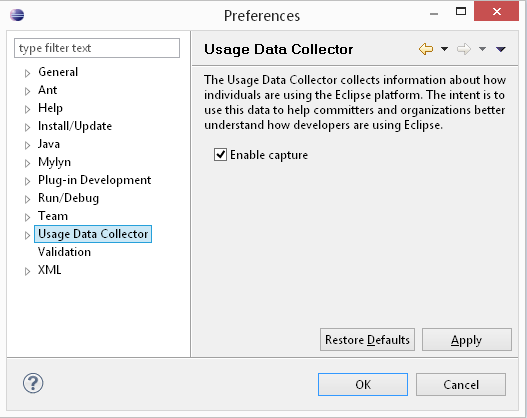
\includegraphics[scale=.58]{26Snipes_prefPage1}
  \caption{Eclipse Usage Data Collector preference page.}\label{fig:prefPage1}
\end{figure}

Before looking at the data, execute a few commands and open a few views
in Eclipse.
Then, on your file system, open the following path as a subdirectory
of your current workspace (Figure~\ref{fig:filesystem}):

\vspace{4mm}
\texttt{.metadata/.plugins/org.eclipse.epp.usagedata.recording}
\vspace{4mm}

\noindent
In that folder, depending on how many UDC events have been gathered,
a number of comma separated value (CSV) files will appear, where \texttt{upload0.csv} is the oldest
and \texttt{usagedata.csv} is the newest.
Open up \texttt{usagedata.csv}---you should notice a large number and a variety of events.
Be sure to look specifically for events that you executed and views that you opened earlier.

\begin{figure}
  \centering
  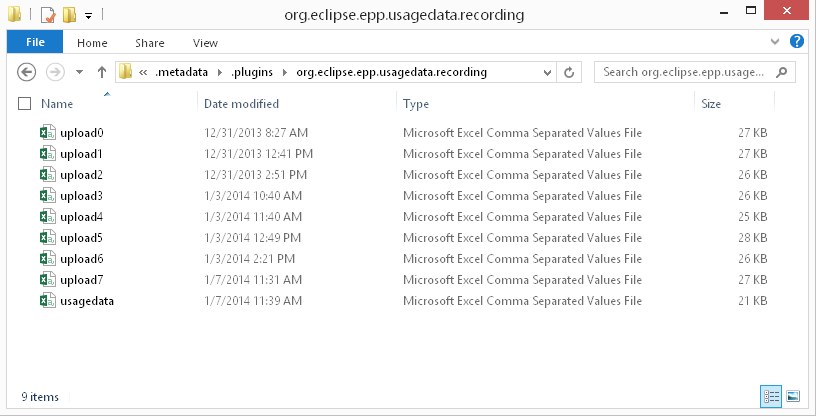
\includegraphics[scale=.58]{26Snipes_filesystem}
  \caption{UDC data files.}\label{fig:filesystem}
\end{figure}

Before doing a study, be aware that Eclipse will ask and periodically attempt to upload
data to the Eclipse foundation server.
You should \emph{not} allow it to do this, because each time data is uploaded, the underlying
CSV files are deleted.
Furthermore, because the UDC project is no longer officially supported, the official Eclipse
UDC server no longer accepts the data, so your usage data is, in effect, lost permanently.
Unfortunately, there is no easy way to tell the UDC client to permanently store
usage data.
An easy workaround is to increase the upload period to 90 days (Figure~\ref{fig:upload}),
which should be enough time to complete the experiment.
The long-term fix for this issue is to either use some other tool, such as
\CodingSpectator{} (\SecRef{CodingSpectator}), to periodically submit the UDC
data to your servers or modify the source code of UDC, as we will explain how to
do shortly, to never upload data.

\begin{figure}
  \centering
  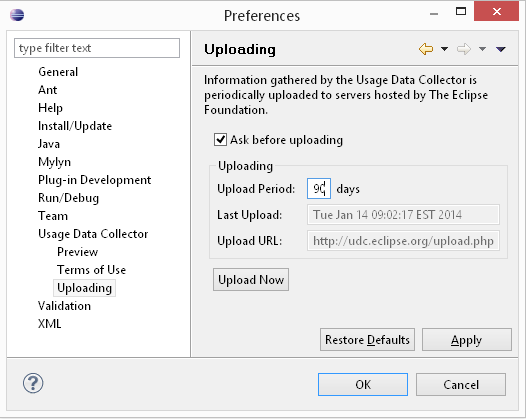
\includegraphics[scale=.58]{26Snipes_upload}
  \caption{Changing the UDC upload frequency.}\label{fig:upload}
\end{figure}

If you're doing a labratory experiment, collecting data should be simply a matter of
copying and deleting the CSV files after each participant has done the experiment.
You can append the files together or put them in a database for analysis.

\paragraph{Modifying the UDC Client.}

You may wish to modify the UDC client yourself, perhaps to add a custom filter for events
or to disable data uploading.
Whatever the reason, making modifications to the client is fairly easy.

The first step is to check out the UDC source code into your Eclipse
workspace using git.\footnote{\url{http://git-scm.com/}}
Here we will again use Eclipse Indigo SR2, but we will specifically be using the
``Eclipse for RCP and RAP Developers'' download package because we will
modify Eclipse plugins.
Before importing the necessary plugins, we recommend switching to
the Indigo SR2 tag, to assure compatibility with
Eclipse.
To do so, clone the git repository\footnote{\url{http://git.eclipse.org/c/epp/org.eclipse.epp.usagedata.git/}}
locally, open up ``Tags'', right click on ``Indigo SR 2'',
then choose ``Checkout''.

To import the projects into Eclipse, right click on the repository, then click
``Import Projects,'' then ``Import Existing Projects.''
The three core projects to import are:

\begin{itemize}
\item org.eclipse.epp.usagedata.internal.gathering
\item org.eclipse.epp.usagedata.internal.recording
\item org.eclipse.epp.usagedata.internal.ui
\end{itemize}

Next, we recommend a quick smoke test to determine whether you
can actually make changes to the UDC client.
Open \texttt{UsageDataRecordingSettings.java}, then modify the value of \texttt{UPLOAD\_URL\_DEFAULT}
to \texttt{"my\_changed\_server"}.
Then, create a new debug configuration that is an Eclipse Application, and press
``Debug'' (Figure~\ref{fig:debugconfig}).
Finally, you can verify that your change worked by going to UDC's Uploading
preference page, noticing that the Upload URL is now ``my\_changed\_server''.

\begin{figure}
  \centering
  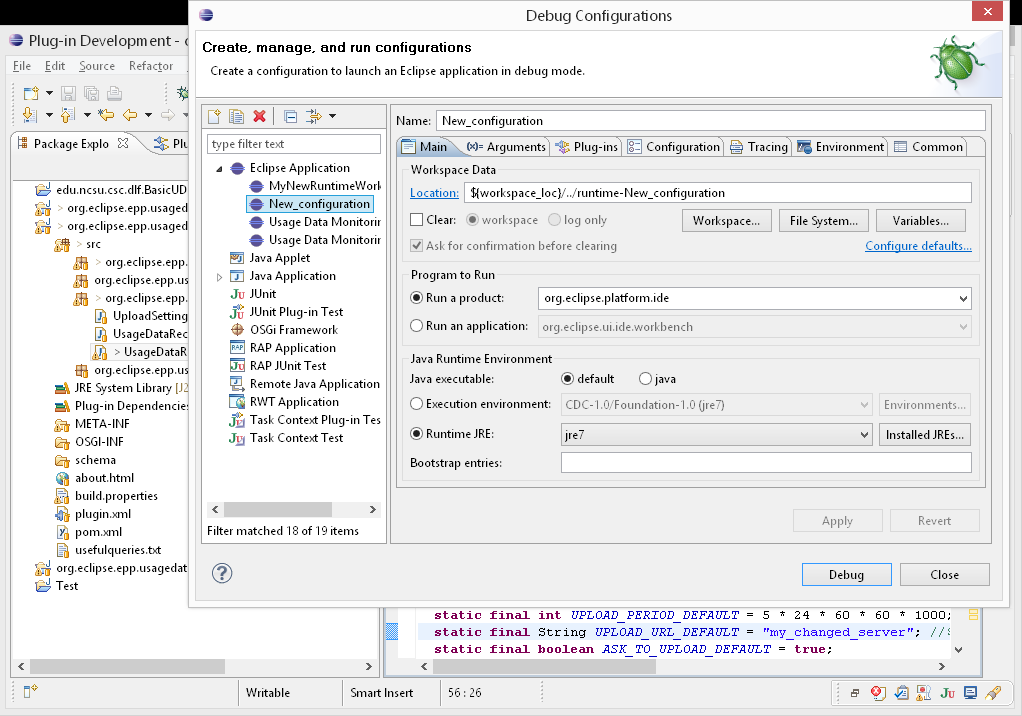
\includegraphics[scale=.58]{26Snipes_debugconfig}
  \caption{Debugging the UDC client.}\label{fig:debugconfig}
\end{figure}

From here, you can make any changes to the UDC client that you wish.
One thing you may want to do is upgrade UDC to work with more recent versions
of Eclipse.
The code is likely currently out of date
because it has not been maintained since the UDC project was shut down.
Another thing you may wish to do is deploy your new version of UDC via
an Eclipse update site to the developers you want to study.
There are many resources on the web for plugin deployment instructions,
such as Lars Vogel's tutorial on creating
plugins.\footnote{\url{http://www.vogella.com/tutorials/EclipsePlugIn/article.html\#deployplugin\_tutorial}}

\paragraph{Transmitting Data over the Internet.}

If you do not plan on doing a lab study where you can manually collect UDC usage
files, you will want to have the UDC client send the data to you directly.
As we mentioned, the best way to do this is probably by changing the default
server URL in the client source code.
An easy way to change the server when debugging is by adding the following Java
virtual machine arguments:

\vspace{4mm}
\texttt{-Dorg.eclipse.epp.usagedata.recording.upload-url=http://localhost:8080}
\vspace{4mm}

\noindent
However, simply changing the client to point at a new URL is insufficient,
because there actually has to be a working server at that URL, ready to
receive UDC data.
%%WBS: It is a bit confusing to talk about the PHP code as not working then talk about the server based on apache.  Why both?
While the source code of official Eclipse server was not officially made
available, Wayne Beaton from the Eclipse Foundation unofficially released
some of the PHP code from the Eclipse Foundation's server.\footnote{\url{https://bugs.eclipse.org/bugs/show_bug.cgi?id=221104}}
Since our PHP skills are rusty, next we'll discuss how to create our own 
server using Java.

Creating your own server that receives UDC data is fairly straightforward.
Let's create a simple one using Apache's HttpComponents library,
the same library that UDC uses to upload data.
Specifically, we can create a server by simply extending Apache's tutorial
web server.\footnote{\url{http://hc.apache.org/httpcomponents-core-ga/httpcore/examples/org/apache/http/examples/ElementalHttpServer.java}}
You can find this server in our github repository.\footnote{\url{https://github.com/wbsnipes/Teufelsberg}}

First, we'll need a generic request handler to wait for HTTP connections:

\begin{lstlisting}
import java.io.IOException;
import org.apache.http.ConnectionClosedException;
import org.apache.http.HttpException;
import org.apache.http.HttpServerConnection;
import org.apache.http.protocol.BasicHttpContext;
import org.apache.http.protocol.HttpContext;
import org.apache.http.protocol.HttpService;

/**
 * Based on
 * http://hc.apache.org/httpcomponents-core-ga/httpcore/examples/org/apache
 * /http/examples/ElementalHttpServer.java
 */
class WorkerThread extends Thread {

	private final HttpService httpservice;
	private final HttpServerConnection conn;

	public WorkerThread(final HttpService httpservice, final HttpServerConnection conn) {
		super();
		this.httpservice = httpservice;
		this.conn = conn;
	}

	@Override
	public void run() {
		System.out.println("New connection thread");
		HttpContext context = new BasicHttpContext(null);
		try {
			while (!Thread.interrupted() && this.conn.isOpen()) {
				this.httpservice.handleRequest(this.conn, context);
			}
		} catch (ConnectionClosedException ex) {
			System.err.println("Client closed connection");
		} catch (IOException ex) {
			System.err.println("I/O error: " + ex.getMessage());
		} catch (HttpException ex) {
			System.err.println("Unrecoverable HTTP protocol violation: " + ex.getMessage());
		} finally {
			try {
				this.conn.shutdown();
			} catch (IOException ignore) {
			}
		}
	}
}
\end{lstlisting}

\newpage
\noindent
We'll also need a generic request listener:

\begin{lstlisting}
import java.io.IOException;
import java.io.InterruptedIOException;
import java.net.ServerSocket;
import java.net.Socket;

import org.apache.http.HttpConnectionFactory;
import org.apache.http.HttpServerConnection;
import org.apache.http.impl.DefaultBHttpServerConnection;
import org.apache.http.impl.DefaultBHttpServerConnectionFactory;
import org.apache.http.protocol.HttpService;

/**
 * Based on
 * http://hc.apache.org/httpcomponents-core-ga/httpcore/examples/org/apache
 * /http/examples/ElementalHttpServer.java
 */
class RequestListenerThread extends Thread {

	private final HttpConnectionFactory<DefaultBHttpServerConnection> connFactory;
	private final ServerSocket serversocket;
	private final HttpService httpService;

	public RequestListenerThread(final int port, final HttpService httpService)
			throws IOException {
		this.connFactory = DefaultBHttpServerConnectionFactory.INSTANCE;
		this.serversocket = new ServerSocket(port);
		this.httpService = httpService;
	}

	@Override
	public void run() {
		System.out.println("Listening on port " + this.serversocket.getLocalPort());
		while (!Thread.interrupted()) {
			try {
				// Set up HTTP connection
				Socket socket = this.serversocket.accept();
				System.out.println("Incoming connection from" + socket.getInetAddress());
				HttpServerConnection conn = this.connFactory.createConnection(socket);

				// Start worker thread
				Thread t = new WorkerThread(this.httpService, conn);
				t.setDaemon(true);
				t.start();
			} catch (InterruptedIOException ex) {
				break;
			} catch (IOException e) {
				System.err.println("I/O error initialising connection thread: " + e.getMessage());
				break;
			}
		}
	}
}
\end{lstlisting}

\newpage
\noindent
And finally, the guts of our server:

\begin{lstlisting}
import java.io.IOException;
import org.apache.http.HttpEntityEnclosingRequest;
import org.apache.http.HttpException;
import org.apache.http.HttpRequest;
import org.apache.http.HttpResponse;
import org.apache.http.protocol.HttpContext;
import org.apache.http.protocol.HttpProcessor;
import org.apache.http.protocol.HttpProcessorBuilder;
import org.apache.http.protocol.HttpRequestHandler;
import org.apache.http.protocol.HttpService;
import org.apache.http.protocol.ResponseConnControl;
import org.apache.http.protocol.ResponseContent;
import org.apache.http.protocol.ResponseDate;
import org.apache.http.protocol.ResponseServer;
import org.apache.http.protocol.UriHttpRequestHandlerMapper;
import org.apache.http.util.EntityUtils;

/**
 * Based on
 * http://hc.apache.org/httpcomponents-core-ga/httpcore/examples/org/apache
 * /http/examples/ElementalHttpServer.java
 */
public class BasicUDCServer {

		public static void main(String[] args) throws IOException {

		int port = 8080;

		HttpProcessor httpproc = HttpProcessorBuilder.create()
				.add(new ResponseDate()).add(new ResponseServer())
				.add(new ResponseContent()).add(new ResponseConnControl()).build();

		UriHttpRequestHandlerMapper reqistry = new UriHttpRequestHandlerMapper();
		reqistry.register("*", new HttpRequestHandler() {

			public void handle(HttpRequest request, HttpResponse response,
					HttpContext context) throws HttpException, IOException {

				HttpEntityEnclosingRequest entityRequest = (HttpEntityEnclosingRequest) request;

				String userID = request.getHeaders("USERID")[0].getValue();
				String workspaceID = request.getHeaders("WORKSPACEID")[0].getValue();
				long time = Long.parseLong(request.getHeaders("TIME")[0].getValue());

				System.out.println(userID + "," + workspaceID + "," + time);
				System.out.println(EntityUtils.toString(entityRequest.getEntity()));
			}
		});

		HttpService httpService = new HttpService(httpproc, reqistry);

		Thread t = new RequestListenerThread(port, httpService);
		t.setDaemon(false);
		t.start();
	}
}
\end{lstlisting}

\noindent
When this server is running and it receives a UDC upload,
it will print a UserId, WorkspaceId, and the time of the upload.
UserIds are randomly generated on the client side and stored in a file in
the developer's home directory.
As long as that file remains intact, future uploads from that developer will
contain that UserId.
WorkspaceIds are identifiers contained in each workspace, and can be
used to uniquely (but anonymously) identify which
workspace a set of data is uploaded from.
Thus, there is normally only one UserId per computer, but there can
be multiple WorkspaceIds per computer.

While there is some coding involved, setting up the UDC for Eclipse can provide thorough usage data collection for a research project using Eclipse.   For lab studies, not much setup is required.  For larger or distributed studies, some infrastructure (a web server) and code (the UDC data server) are required.  Next we look at Mylyn and the Eclipse Mylyn Monitor component.

\subsection{Mylyn and the Eclipse Mylyn Monitor}
\label{MylynMonitor}

%\usepackage{color}
\definecolor{darkblue}{rgb}{0.0,0.0,0.6}
\definecolor{cyan}{rgb}{0.0,0.6,0.6}
\definecolor{maroon}{rgb}{0.5,0,0}
\definecolor{darkgreen}{rgb}{0,0.5,0}


%Mylyn~\cite{mylyn-web,Kersten-Mylar2005,Kersten-Mylyn,kersten2007focusing} is a task focused user interface, a top-level project of the Eclipse IDE that is part of many of the Eclipse IDE configurations. To better support developers in managing and working on multiple tasks, Mylyn makes tasks a first class entity, monitors a developer's interaction with the IDE for each task and logs it in a so-called \textit{task context}.

\citeasnoun{Kersten-Mylyn} created Mylyn, a task focused user interface, a top-level project of the Eclipse IDE that is part of many of the Eclipse IDE configurations. To better support developers in managing and working on multiple tasks, Mylyn makes tasks a first class entity, monitors a developer's interaction with the IDE for each task and logs it in a so-called \textit{task context}.

%The first versions of Mylyn, originally called Mylar, were developed as part of the PhD research of Mik Kersten and contained an explicit Mylyn Monitor component to collect and upload a developer's activity within the Eclipse IDE~\cite{mylyn-monitor}. While the source code of the Mylyn Monitor can still be found on-line, it is not an active part of the Mylyn project anymore.
The first versions of Mylyn, originally called Mylar, were developed as part of the PhD research of Mik Kersten and contained an explicit Mylyn Monitor component to collect and upload a developer's activity within the Eclipse IDE. While the source code of the Mylyn Monitor can still be found on-line, it is not an active part of the Mylyn project anymore.

\subsubsection{Collected Data}
Mylyn captures three types of developer interactions with the Eclipse development environment:
\begin{itemize}
    \item the \textit{selection} of elements,
    \item the \textit{editing} of elements, and
    \item \textit{commands} in the IDE, such as saving or refactoring commands.
\end{itemize}

These interaction events are monitored and then stored in XML format in a log file. An interaction event log example of a developer selecting a Java class \texttt{TaskEditorBloatMonitor.java} in the package explorer of the Eclipse IDE is:

\lstdefinelanguage{XML}
{
  basicstyle=\ttfamily,
  morestring=[s]{"}{"},
  morecomment=[s]{?}{?},
  morecomment=[s]{!--}{--},
  commentstyle=\color{darkgreen},
  moredelim=[s][\color{darkblue}]{>}{<},
  moredelim=[s][\color{red}]{\ }{=},
  stringstyle=\color{blue},
  identifierstyle=\color{maroon},
  morekeywords={StructureKind}
}


\lstset{
  language=XML,
  columns=fullflexible,
  showstringspaces=false,
  commentstyle=\color{gray}\upshape
}


\begin{lstlisting}
<InteractionEvent 
    StructureKind="java"
    StructureHandle="=org.eclipse.mylyn.tasks.ui/src&lt;org.eclipse.mylyn.
        internal.tasks.ui{TaskEditorBloatMonitor.java" 
    StartDate="2012-04-10 02:05:53.451 CEST"
    OriginId="org.eclipse.jdt.ui.PackageExplorer" 
    Navigation="null" 
    Kind="selection" 
    Interest="1.0" 
    EndDate="2012-04-10 02:05:53.451 CEST" 
    Delta="null"
/>
\end{lstlisting}

The log entry contains among other information the interaction event kind, in this case a selection, the full identifier of the element the developer interacted with, a Java type called TaskEditorBloatMonitor, the time when the interaction event occurred, in this case October 4th, 2012, at 02:05:52 CEST, and the place where the interaction event occurred, in this case the package explorer view of Eclipse. 

You may notice that the log also contains an interest value, in this case 1.0. This value is used by Mylyn to calculate the interest a developer shows in a code element, the so-called degree-of-interest. The degree-of-interest of a code element, such as a class, method or field, is based on the recency and frequency of interactions while working on a task. The more frequent and recent a developer selected and/or edited a code element, the higher the degree-of-interest. This degree-of-interest value is then used to highlight and/or filter elements in views of the IDE ~\citeaffixed{kersten2007focusing,Kersten-Mylyn}{see}.

The Mylyn Usage Monitor developed for the original research project and study, writes the interaction events sequentially into the interaction log file, while the developer is interacting with the IDE. The monitor that is used in later versions of Mylyn, including the current one, compresses the log for performance reasons and aggregates interaction events where possible. The compression looses the information on the time sequence and it is not possible to fully reconstruct the order and exact time in which each interaction event occurred. Since the task context in Mylyn is mainly used for calculating the degree-of-interest of an element, the exact time order is not necessary.


\subsubsection{Logging Interactions with the Mylyn Monitor}
	While the code for the Mylyn Monitor is not part of the active Mylyn project anymore, the code for the monitor and example code for using it can be found in the incubator project online\footnote{\url{http://git.eclipse.org/c/mylyn/org.eclipse.mylyn.incubator.git/tree/}} \footnote{\url{http://wiki.eclipse.org/Mylyn_Integrator_Reference\#Monitor_API}}. In the following, we will present relevant parts of the code from these examples to log the interactions.

To be able to use the Mylyn Monitor code and log the events of interest there are two important classes you have to implement. First, you will need a plug-in class that extends 
the following plugin: 

\begin{lstlisting}
org.eclipse.ui.plugin.AbstractUIPlugin
\end{lstlisting}

\noindent
Then, add a listener for the events that you are interested in to:

\begin{lstlisting}
org.eclipse.mylyn.internal.monitor.ui.MonitorUiPlugin 
\end{lstlisting}

Second, you will need to write the listener that creates the interaction event objects when an interaction event occurs. Let's assume you want to write a listener for selections of Java elements in the IDE. In this case you can extend the class \texttt{org.eclipse.mylyn.monitor.ui.AbstractUserInteractionMonitor} and simply override the \texttt{selectionChanged} method. By extending the \texttt{AbstractUserInteractionMonitor}, your listener will automatically be added as a post selection listener to all windows in the current workbench so that all selection events in the windows are forwarded to your listener. The relevant code for the \texttt{selectionChanged} method is:


% Revert list settings
\lstset{language=Java,
captionpos=b,
tabsize=3,
frame=lines,
numbers=left,
numberstyle=\tiny,
numbersep=5pt,
breaklines=true,
showstringspaces=false,
basicstyle=\footnotesize,
emph={label}}

\begin{lstlisting}
/** 
 * Based on
 * http://git.eclipse.org/c/mylyn/org.eclipse.mylyn.incubator.git/tree/
 * org.eclipse.mylyn.examples.monitor.study/src/org/eclipse/mylyn/examples/
 * monitor/study/SelectionMonitor.java
 */
import org.eclipse.jface.viewers.ISelection;
import org.eclipse.jface.viewers.StructuredSelection;
import org.eclipse.mylyn.monitor.core.InteractionEvent;
import org.eclipse.jdt.core.IJavaElement;

...

    @Override
    public void selectionChanged(IWorkbenchPart part, ISelection selection) {
		InteractionEvent.Kind interactionKind = InteractionEvent.Kind.SELECTION;
		if (selection instanceof StructuredSelection) {
			StructuredSelection structuredSelection = (StructuredSelection) selection;
			Object selectedObject = structuredSelection.getFirstElement();
			if (selectedObject == null) {
				return;
			}

			if (selectedObject instanceof IJavaElement) {
				IJavaElement javaElement = (IJavaElement) selectedObject;
				structureKind = STRUCTURE_KIND_JAVA;
				elementHandle = javaElement.getHandleIdentifier();
			}
		}

		...

		InteractionEvent event = new InteractionEvent(interactionKind, structureKind,
                                elementHandle, ...);
		MonitorUiPlugin.getDefault().notifyInteractionObserved(event);
	}

...
\end{lstlisting}

The code first checks what type the selection has. If the selection is structured, and the first part of it is a Java Element, it collects the relevant information and then creates an \texttt{InteractionEvent} with the gathered information, such as the interaction kind, the structure kind and the element handle. At the end of the method, the \texttt{MonitorUiPlugin} is notified about the observed interaction event. The \texttt{MonitorUiPlugin} will then go through all registered interaction event listeners and forward the event to them. Since there is an \texttt{InteractionEventLogger} registered as part of the Mylyn code, the interaction event object will be forwarded to the logger and then written out into a file. 

%TODO: wrap up the Mylyn section

\subsection{\CodingSpectator}
\label{CodingSpectator}

\CodingSpectator \footnote{\url{http://codingspectator.cs.illinois.edu/}} described by  ~\cite{VakilianETAL2011Richer,VakilianETAL2012UseDisuseMisuse,VakilianETAL2013Compositional}
 is
an extensible framework for collecting Eclipse usage data. Although
researchers at the University of Illinois at Urbana-Champaign
developed \CodingSpectator{} primarily for collecting detailed data
about the use of the Eclipse refactoring tool, it also provides a
reusable infrastructure for \emph{submitting usage data} from developers to
a central repository.  
\CodingTracker \footnote{\url{http://codingtracker.web.engr.illinois.edu/}} described by  ~\cite{NegaraETAL2012Dangerous,NegaraETAL2013ManualRefactorings} is another
data collector developed at Illinois, which collects finer-grained IDE
actions while reusing the data submission infrastructure provided by
\CodingSpectator.

\subsubsection{Collected Data}

\CodingSpectator{} was designed for capturing detailed data about the use of
automated refactorings. It collects three kinds of refactoring events:
\Canceled, \Performed, and \Unavailable. If a programmer starts an automated
refactoring but quits it before it finishes, \CodingSpectator{} records a
\Canceled{} refactoring event. If a programmer applies an automated refactoring,
\CodingSpectator{} records a \Performed{} refactoring event. Finally, if
a programmer invokes an automated refactoring but the IDE refuses to start the
automated refactoring indicating that the refactoring is not applicable to the
selected program element, \CodingSpectator{} records an \Unavailable{}
refactoring event.

Eclipse creates a \emph{refactoring descriptor} object for each \Performed{}
refactoring events and serializes it in an XML file. \CodingSpectator{} saves
more data in Eclipse refactoring descriptors of \Performed{} refactorings. In
addition, it creates and serializes refactoring descriptors for \Canceled{} and
\Unavailable{} refactoring events. \CodingSpectator{} supports
\Use{NumberOfCodingSpectatorSupportedRefactorings} of the
\Use{NumberOfEclipseAutomatedRefactorings} automated refactorings that Eclipse
supports.

We show a concrete example of the data that \CodingSpectator{}
collects for an invocation of the automated Extract Method refactoring
in Eclipse, which extracts a piece of code into a new method. This
refactoring moves a selected piece of code into a new method and
replaces the selected code by an invocation to the new method. To use
the automated Extract Method refactoring, a programmer has to go
through multiple steps. First, the programmer selects a piece of code
(\FigRef{FigCodingSpectatorExtractMethodSelectionExample}). Second,
the programmer invokes the automated Extract Method and configures it
(\FigRef{FigCodingSpectatorExtractMethodConfigurationExample}). In
this case, the programmer sets the name of the new method. The
configuration page provides a number of other options including method
accessibility, the ordering and names of method parameters, and the
generation of method comments. Third, after configuring the
refactoring, the programmer hits the ``Preview'' button and the
automated refactoring reports the problems that the refactoring may
introduce (\FigRef{FigCodingSpectatorExtractMethodErrorExample}). In
this example, the automated refactoring complains that the selected
name of the new method conflicts with the name of an existing
method. Finally, the programmer decides to cancel the refactoring and
\CodingSpectator{} records a refactoring descriptor for this
\Canceled{} refactoring, as shown in
\FigRef{FigCodingSpectatorDescriptorExample}. The type of a
refactoring event (\ie, \Unavailable, \Canceled, and \Performed) can
be inferred from the directory in which the XML file containing the
refactoring descriptor resides.  \CodingSpectator{} captures the
following attributes for the canceled automated Extract Method
refactoring in the above example.

\begin{enumerate}

\item \texttt{captured-by-codingspectator}: indicates that \CodingSpectator{}
  created the refactoring descriptor.

\item \texttt{stamp}: a time-stamp recording when the refactoring event occurred

\item \texttt{code-snippet}, \texttt{selection},
  \texttt{selection-in-code-snippet}, \texttt{selection-text}: the location and
  contents of the selection that the programmer made before invoking the
  automated refactoring

\item \texttt{id}: the automated refactoring's identifier

\item \texttt{comment}, \texttt{description}, \texttt{comments},
  \texttt{destination}, \texttt{exceptions}, \texttt{flags}, \texttt{input},
  \texttt{name}, \texttt{visibility}: configuration options, \eg{} input
  elements, project, and settings that programmers can set to control the effect
  of the refactoring

\item \texttt{status}: any problems reported by the automated refactoring to the
  programmer

\item \texttt{navigation-history}: when the programmer pressed a button to
  navigate from one page of the refactoring wizard to another

\item \texttt{invoked-through-structured-selection},
  \texttt{invoked-by-quick-assist}: selection method (\eg{} structured or
  textual selection and whether the automated refactoring was invoked using
  Quick Assist

\end{enumerate}

\begin{figure}
%
\centering
%
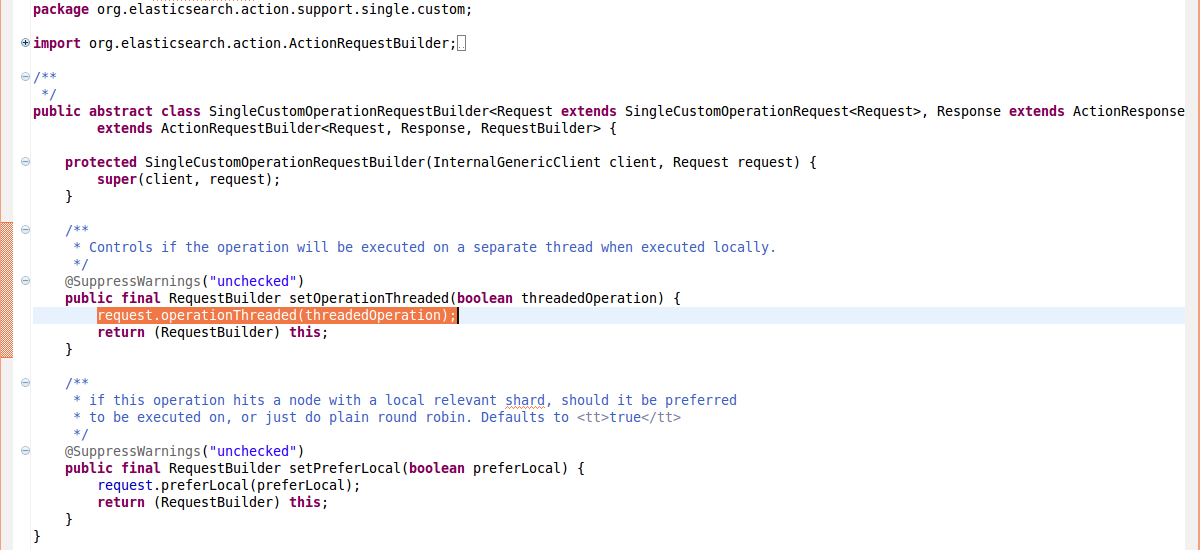
\includegraphics[width=\textwidth]{26Snipes_codingspectator-extract-method-selection.png}
%
\caption{\label{FigCodingSpectatorExtractMethodSelectionExample}A programmer
selects a piece of code to extract into a new method. The selected code is part
of class \texttt{SingleCustomOperationRequestBuilder} from commit
\texttt{bdb1992} of the open-source Elasticsearch project
(\texttt{https://github.com/elasticsearch/elasticsearch}).}
%
\end{figure}

\begin{figure}
%
\centering
%
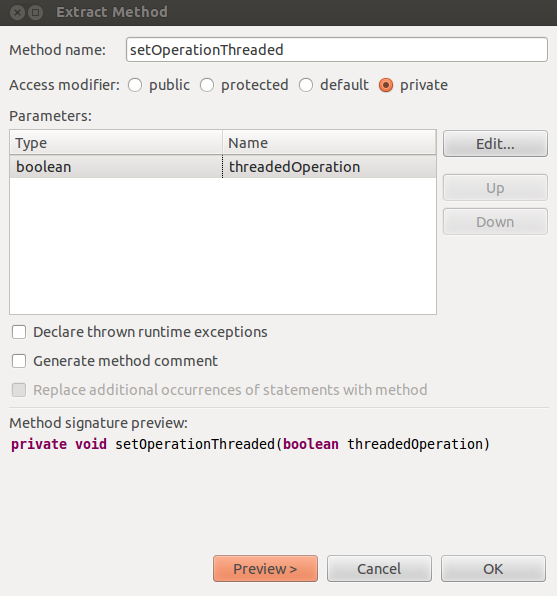
\includegraphics[width=0.5\textwidth]{26Snipes_codingspectator-extract-method-configuration.png}
%
\caption{\label{FigCodingSpectatorExtractMethodConfigurationExample}A programmer
configures an automated Extract Method refactoring by entering the desired name
of the new method.}
%
\end{figure}

\begin{figure}
%
\centering
%
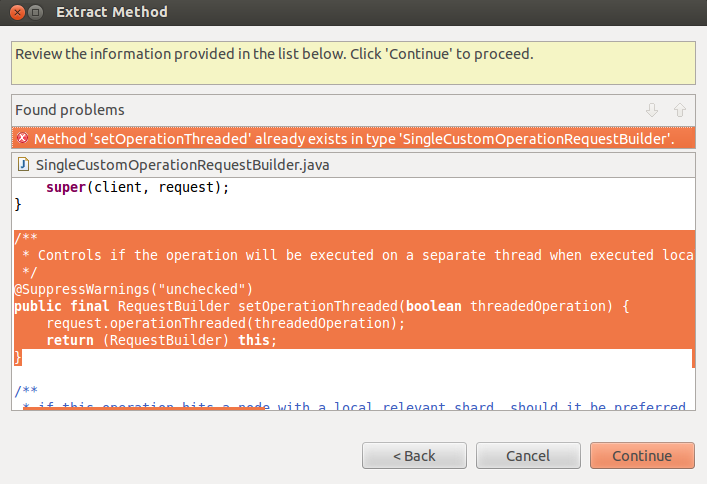
\includegraphics[width=0.6\textwidth]{26Snipes_codingspectator-extract-method-error.png}
%
\caption{\label{FigCodingSpectatorExtractMethodErrorExample}The Extract Method
refactoring reports a name conflict problem to the programmer. The programmer
can either ignore the problem and continue the refactoring, go back to the
configuration page to provide a different name, or cancel the refactoring.}
%
\end{figure}

\begin{figure}
%
\centering
%
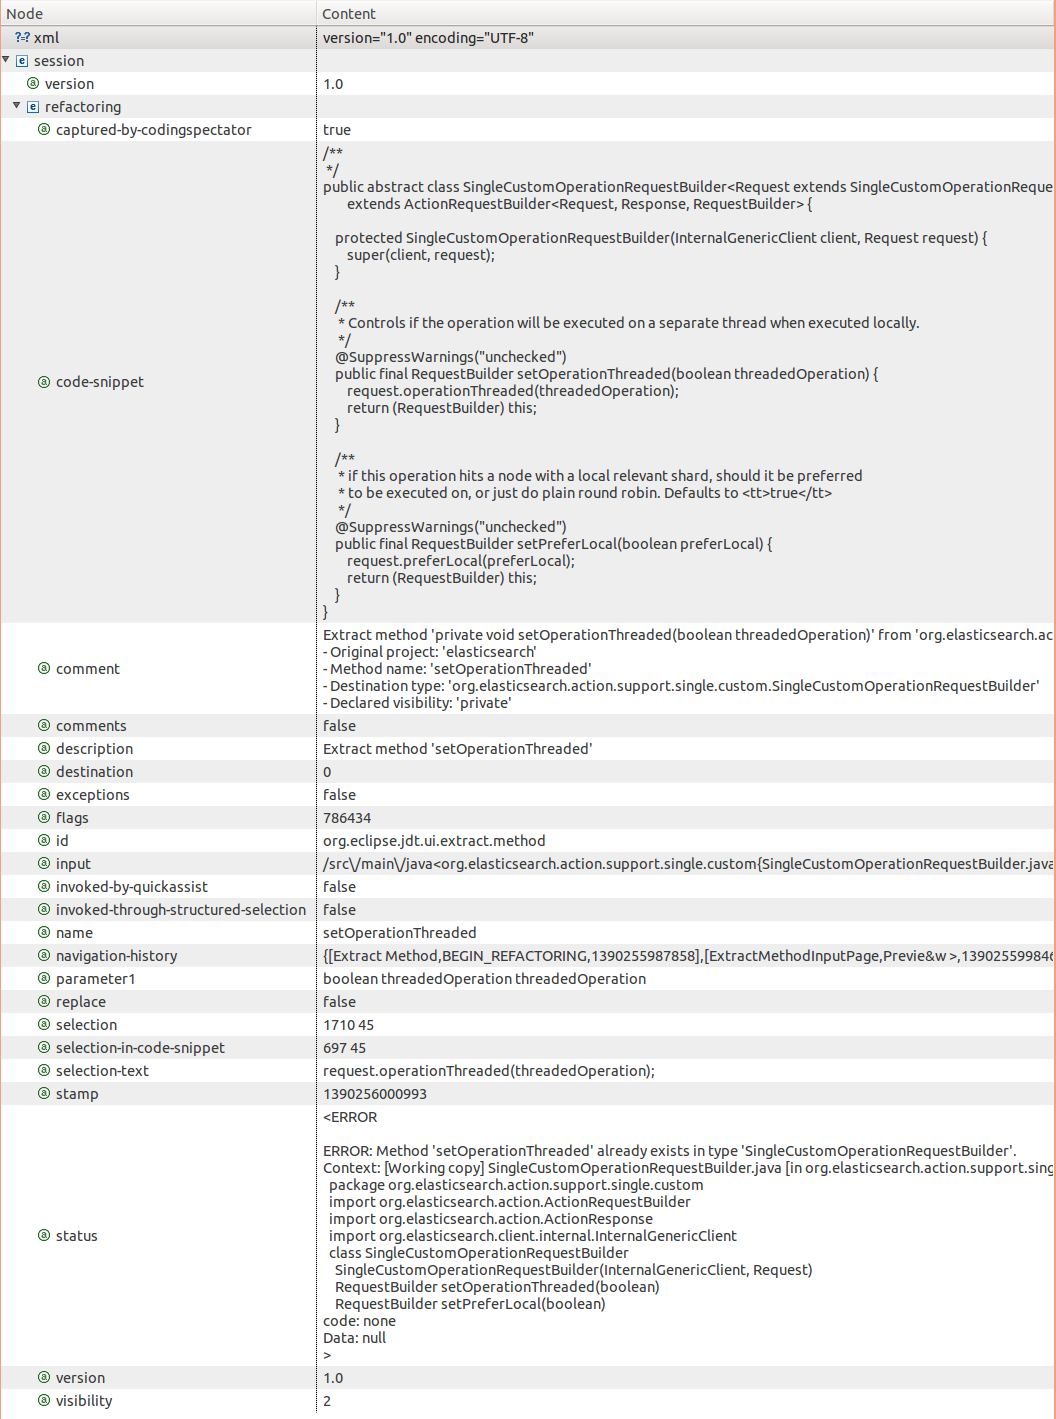
\includegraphics[width=\textwidth]{26Snipes_codingspectator-refactoring-xml.png}
%
\caption{\label{FigCodingSpectatorDescriptorExample}An example refactoring
descriptor recorded by \CodingSpectator.}
%
\end{figure}

\subsubsection{Deploying \CodingSpectator}

Deploying \CodingSpectator{} consists of two main steps:
%
\begin{inparaenum}[(1)]
%
\item setting up a Subversion repository and
%
\item setting up an Eclipse update site.
%
\end{inparaenum}

\begin{enumerate}
\item
\textbf{Setting Up a Subversion Repository -}
\CodingSpectator{} regularly submits developers' data to a central Subversion
repository. To collect \CodingSpectator's data automatically, you need to set up
a Subversion repository and create accounts for your developers. To allow the developers
to submit their data to the Subversion repository, you should grant them
appropriate write accesses to the repository.

Using a Version Control System such as Subversion as the data repository has
several advantages:

\begin{enumerate}
%
\item Subversion makes all revisions of each file easily accessible. This makes
  troubleshooting easier for researchers.
%
\item For textual files, Subversion submits only the \emph{changes} made to the
  files as opposed to the entire new file. This differential data submission
  leads to faster submissions.
%
\item There are libraries such as SVNKit\footnote{http://svnkit.com/} that
  provide an API for Subversion operations such as add, update, remove, and
  commit. \CodingSpectator{} uses SVNKit for submitting developers' data to the
  central repository.
%
\item Setting up a Subversion server is a well-documented process. This avoids
  the burden of setting up a specialized server.
%
\end{enumerate}

On the other hand, a disadvantage of using Subversion as the data repository is
that it requires the developers to maintain a copy of their data on their file
systems. The Subversion working copy on the developers' systems takes \emph{space}
and can also cause \emph{merge conflicts}, \eg, if a developer restores the contents
of the file system to an earlier version. To handle merge conflicts,
\CodingSpectator{} has built-in support for automatic conflict detection and
resolution. When \CodingSpectator{} detects a merge conflict, it removes the
developer's data from the central repository and then submits the new data. Despite
removing the data from the central repository, the researchers can still locate
the merge conflicts and restore the data that was collected before the conflicts occurred.

\CodingSpectator{} prompts the developers for their Subversion user names and
passwords when \CodingSpectator{} is about to submit their data.
\CodingSpectator{} gives the developers the option to save their passwords in Eclipse
securely. See \url{http://codingspectator.cs.illinois.edu/documentation} for
more information about the features of \CodingSpectator{} for developers.

\item
\textbf{Setting Up an Eclipse Update Site -}
Users of \CodingSpectator{} install it from an Eclipse update
site\footnote{\url{http://codingspectator.cs.illinois.edu/installation}}. An
Eclipse update site is an online repository of the JAR and configuration files
that Eclipse requires for installing a plug-in.

You will have to customize \CodingSpectator{} at least by specifying the URL of
the Subversion repository to which \CodingSpectator{} should submit developers' data.
You may also want to customize the message that \CodingSpectator{} shows to the
developers when it prompts them for their Subversion credentials. You can customize
these aspects of \CodingSpectator{} by changing the configuration files that are
packed in the existing JAR files hosted at the Eclipse update site of
\CodingSpectator. If you need to customize \CodingSpectator{} in more complex
ways that involve changes to its source code, you should follow the instructions
for building \CodingSpectator's update site from source code.
\end{enumerate}

\subsubsection{Extending \CodingSpectator}

In addition to collecting detailed refactoring data, \CodingSpectator{} provides
a reusable infrastructure for collecting Eclipse usage data. Extending
\CodingSpectator{} frees researchers from having to develop many features from
scratch, \eg, Subversion communications, automatic merge conflict detection and
resolution, secure storage of Subversion credentials, and periodic update
reminders.

\CodingSpectator{} provides an Eclipse extension point (id =
\texttt{edu.\-illinois.\-codingspectator.\-monitor.\-core.\-submitter}) and the
following interface:

\begin{lstlisting}
public interface SubmitterListener {
  // hook before svn add
  void preSubmit();
  // hook after svn add and before svn commit
  void preCommit();
  // hook after svn commit
  void postSubmit(boolean succeeded);
}
\end{lstlisting}

The above interface provides three hooks to \CodingSpectator's submission
process. \CodingSpectator{} checks out the Subversion repository into a folder,
which we refer to as the \emph{watched folder}. Then, it executes the Subversion
commands (\eg, add and commit) on the watched folder. A plug-in that extends the
\Code{submitter} extension point and implements the \Code{SubmitterListener}
interface can perform actions before or after two of the Subversion commands that
\CodingSpectator{} executes: add and commit.
%
For example, \CodingSpectator{} overrides the method \Code{preSubmit} to copy
the recorded refactoring descriptors to the watched folder. As another example,
the developers of \CodingSpectator{} made the Eclipse UDC plug-in use the
\Code{submitter} extension point and copy the UDC data to the watched folder. As
a result, \CodingSpectator{} submits the UDC data to the Subversion repository.
Effectively, this is an alternative method to the one presented in
\SecRef{SecUDCHowToUseIt} for collecting UDC data in a central repository.

% LocalWords: CodingSpectator Urbana Champaign IDE timestamp
%
% LocalWords: CodingTracker refactoring refactorings refactoring's
%
% LocalWords: SVNKit URL usernames online API


\subsection{Build it Yourself for Visual Studio}
\label{buildItYourself}

This section shows how to implement a usage data collection tool for Visual Studio that generates the Navigation Ratio metric (see section \ref{SelectingData}) daily, giving the developer insight into his own navigation patterns. Readers attempting the tutorial should be familiar with C\# as well as have a working knowledge of Visual Studio.  

Because this extension is illustrative some simplifications have been made that would need to be addressed in a widely deployed extension. For instance, this example extension does not perform any background processing, thus the developer may notice a delay during Visual Studio startup.  

\subsubsection{Creating a Visual Studio Extension}

To add functionality to Visual Studio we must utilize the extensibility platform, creating a Visual Studio Extension. Once the extension is created we can add our specific functionality.

\begin{enumerate}
\item {\bf Install the Visual Studio SDK} - To create Visual Studio Extensions specialized libraries (e.g., the automation library) are needed, and thus the Visual Studio SDK must be installed.

\item {\bf Create a Visual Studio Solution and Project} - Using the ``New Project'' wizard create a new project and solution in C\# by selecting Extensibility and Visual Studio Packageas shown in Figure \ref{fig:ProjectCreation}.  
\begin{figure}
	\centering
	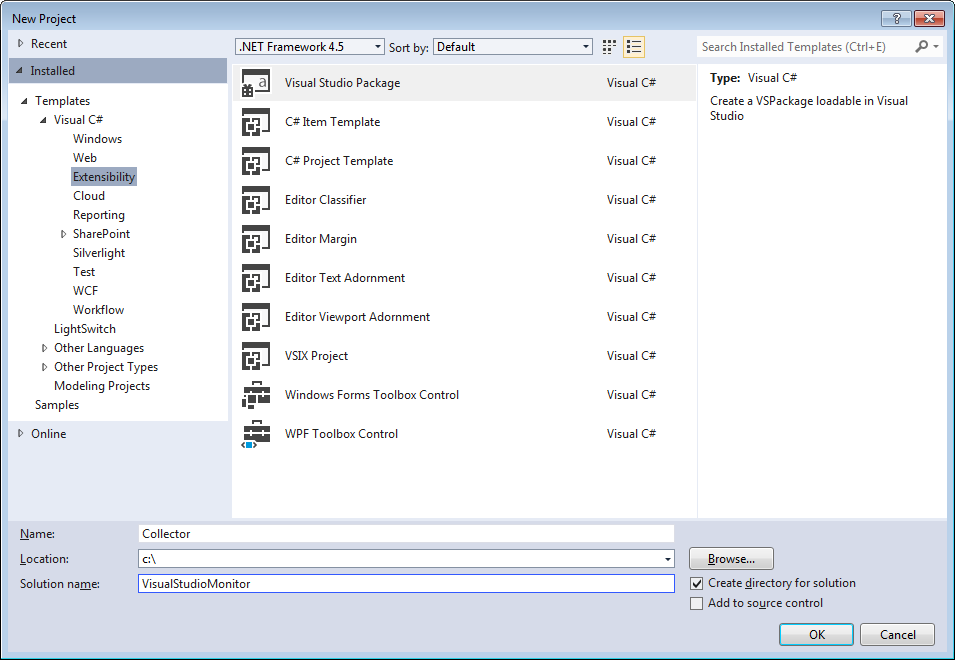
\includegraphics[width=4in]{26Snipes_CreateVSIXExtension.png}
	\caption{Create a Visual Studio Extension}
	\label{fig:ProjectCreation}
\end{figure}

Use ``Collector'' as the project name and ``VisualStudioMonitor'' as the solution name, then follow the default options for the first 2 steps of the wizard.  In the third step, when asked to specify what type of extension, select the option to generate a menu command.  Next, give the menu command a name of "Stop Monitoring" and a command ID of ``StopMonitoring''.  This menu option will allow the developer to halt collection of data if they wish without quitting Visual Studio.  Click next on the next step and then Finish to setup your extension solution project.


After creating the project and solution, the solution explorer should look like figure \ref{fig:SolutionExplorer} showing the project files necessary for the extension to work.
\begin{figure}
	\centering
	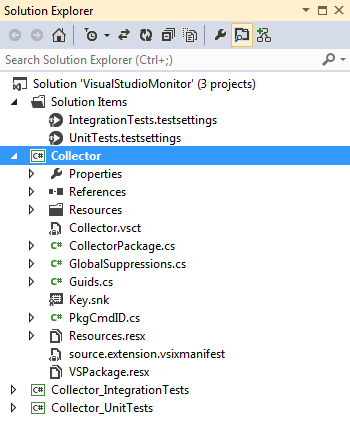
\includegraphics[width=2.5in]{26Snipes_SolutionExplorer.png}
	\caption{Solution Explorer with Visual Studio Extension}
	\label{fig:SolutionExplorer}
\end{figure}


\item {\bf Ensure the extension loads on startup} - The next step is to instruct the extension package to load when Visual Studio starts, by setting the attribute ProvideAutoLoad on the package class (CollectorPackage.cs). The GUID value in the below listing will load the package when Visual Studio starts.

\begin{lstlisting}
    // This attribute starts the package when Visual Studio starts 
    [ProvideAutoLoad("{ADFC4E64-0397-11D1-9F4E-00A0C911004F}")]
    [Guid(GuidList.guidCollectorPkgString)]
    public sealed class CollectorPackage : Package
\end{lstlisting}

\end{enumerate}

\subsubsection{Create Monitor Project}

To separate the Visual Studio Extension setup code from the core functionality of the extension a second project should be created within the same solution. We call this second project  the Monitor project.

\begin{enumerate}
\item {\bf Create the Monitor project} - Add a class library type project to  the "VisualStudioMonitor" solution. Because the class library must be signed, go to the Properties for the Monitor project and select Signing from the list at the right.  In the Signing tab, check the "sign the assembly" checkbox then under "Choose a strong name key file", select Browse and browse over to the Key.snk file in the collector project (the file was created with the solution).

\item {\bf Create the monitoring class} - 
The next step is to create a static class that will manage the log file including starting, stopping recording data, and inserting data into the log file.  Rename the class created by Visual Studio in the Monitor project to "DataRecorder".    Because we don't want more than one recorder running at a time and want to access this class without instantiating it, make the class static.  Create a method to Start the recorder that generates a file name for the log file and sets a flag that the recording has started. A Stop method resets that flag and perhaps clears the file name.  A method to write a log message to the file completes DataRecorder.

\item {\bf Connecting the extension framework with the recorder} -
Finally, insert a call to DataRecorder.Start() at the end of the Initialize() method in the CollectorPackage class.  This will start the monitoring each time Visual Studio starts.  You will need to add a reference for the "Monitor" project to the Collector project, make sure you sign the Monitor project, then rebuild the solution.


The call to DataRecorder.Start() is inserted in the CollectorPackage as shown in Listing \ref{code:StartCall}.
\begin{lstlisting}[caption=Call to DataRecorder.Start(),label=code:StartCall]
        /////////////////////////////////////////////////////////////////////////////
        // Overridden Package Implementation
        #region Package Members

        /// <summary>
        /// Initialization of the package; this method is called right after the package is sited, so this is the place
        /// where you can put all the initialization code that rely on services provided by VisualStudio.
        /// </summary>
        protected override void Initialize()
        {
            Debug.WriteLine (string.Format(CultureInfo.CurrentCulture, "Entering Initialize() of: {0}", this.ToString()));
            base.Initialize();

            // Add our command handlers for menu (commands must exist in the .vsct file)
            OleMenuCommandService mcs = GetService(typeof(IMenuCommandService)) as OleMenuCommandService;
            if ( null != mcs )
            {
                // Create the command for the menu item.
                CommandID menuCommandID = new CommandID(GuidList.guidCollectorCmdSet, (int)PkgCmdIDList.StopCollector);
                MenuCommand menuItem = new MenuCommand(MenuItemCallback, menuCommandID );
                mcs.AddCommand( menuItem );
            }
            DataRecorder.Start();
        }
        #endregion
\end{lstlisting}

The source code for the DataRecorder.cs file is shown in Listing \ref{code:DataRecorder}
\begin{lstlisting}[caption=Data Recorder Class,  label=code:DataRecorder]
using System;
using System.Collections.Generic;
using System.Linq;
using System.Text;
using System.Threading.Tasks;

namespace Monitor
{
    public static class DataRecorder
    {
        public static void Start() {
            logDirectoryPath = System.IO.Path.GetTempPath();
            logFileName = System.IO.Path.Combine(logDirectoryPath, "collector " + DateTime.Now.ToString("yyyy-MM-dd HH.mm.ss") + ".log");
            try {
                using (System.IO.StreamWriter streamWriter = new System.IO.StreamWriter(
                    new System.IO.FileStream(logFileName, System.IO.FileMode.OpenOrCreate, System.IO.FileAccess.Write, System.IO.FileShare.ReadWrite)
                    ))
                {
                    streamWriter.WriteLine("Collector Started");
                }
            } 
            catch (System.IO.IOException ioexception) {
                Console.WriteLine("Error creating log file "+ioexception);
            }
         }

        public static void Stop() {

                WriteLog("Collector Stopped");
            
        
        }

        public static void WriteLog(string logToWrite)
        {
            try
            {
                using (System.IO.StreamWriter streamWriter = new System.IO.StreamWriter(
                    new System.IO.FileStream(logFileName, System.IO.FileMode.Append, System.IO.FileAccess.Write, System.IO.FileShare.ReadWrite)
                    ))
                {
                    streamWriter.WriteLine(logToWrite);
                }
            }
            catch (System.IO.IOException ioexception)
            {
                Console.WriteLine("Error writing to log file " + ioexception);
            }
        
        }

        private static string logFileName;
        private static string logDirectoryPath;
    }
}

\end{lstlisting}
\end{enumerate}

\subsubsection{Create the Data Model}

The next step creates a data model for storing and managing event monitoring for Visual Studio. This includes designing the main event types and implementing a factory to create these events. 

%Because there are several different types of events, it makes sense to build an abstract class to manage the core data and use the Simple Factory pattern to generate each type of event monitoring.  With this pattern an abstract base class, called AbstractMonitoredEvent, provides common definitions for class fields that will be used for monitoring different Visual Studio events, conversion of those fields to and from the storage format, and (eventually) calling the WriteLog method in the recorder when the event fires.  This concrete class implements methods specific to Visual Studio commands that manages the fields available from the DTE.Command class.  The client in the Simple Factory pattern is a class that maintains the collection of events that either gets read from the file or queried from Visual Studio.   In this step we focus on the elements needed to store event information, and manage the configuration file data in XML format.

\begin{enumerate}
\item {\bf Implement the base class} - 
Create the AbstractMonitoredEvent class in the Monitor project in Visual Studio.  Then add data elements for EventName and Classification as follows.

\begin{lstlisting}
    [XmlInclude(typeof(MonitoredCommandEvent))]
    [XmlRoot(ElementName = "MonitoredEvent", Namespace = "http://Monitor")]
    public abstract class AbstractMonitoredEvent
    {
        /// <summary>
        /// Default constructor to use in serialization
        /// </summary>
        protected AbstractMonitoredEvent()
        {
        }

        public String EventName { get; set; }
        public String Classification { get; set; }
   }
\end{lstlisting}

\item {\bf Enable serialization in base class} - 
So that we can store events in a configuration file then manipulate that configuration file later, we provision this abstract class for XML serialization of itself and its derived classes.  Dot NET attributes support the XML serialization in this structure.  The first attribute tells XML serialization that the MonitoredCommandEvent class is a derived class of AbstractMonitoredEvent that we will create next.  This provides the abiltiy to serialize and deserialize the public objects of the derived class by referencing the type of AbstractMonitoredEvent when creating a serializer.  The second attribute creates an XML namespace that all derived classes will share with the AbstractMonitoredEvent class.

\item {\bf Create the concrete subclass} - 
The next step is to create a derived class called MonitoredCommandEvent that inherits from AbstractMonitoredEvent.  MonitoredCommandEvent implements a constructor that builds a MonitoredCommandEvent object from the Command class of the DTE.

The EnvDTE.Command object contains fields for Guid (a GUID string), ID and integer sub-id, and Name a readable name for the command.  To register an event handler for a EnvDTE.Command, you need get an object reference for the command using the Guid and ID to identify the command.  The GUID is  a Globally Unique IDentifier for command events in Visual Studio, however, some command events share a GUID and distinguish themselves with different EventIDs. Thus both elements are necessary to link a Command event from the DTE to an event hander in this extension.  The Name is useful information to understand what the command is.    There are several versions of the DTE object corresponding to versions of Visual Studio.  Depending on the commands of interest, each version may need to be queried for its commands.  

 The constructor that takes a Command as input, simply extracts the necessary and relevant fields from the DTE's Command object and transferrs the matching information into the corresponding fields from this class and the AbstractMonitoredEvent class.  

\item {\bf Enable serialization in concrete subclass} -
Ensure the class also includes a constructor that builds from an XElement and an output method ToXElement translates the object to XML for saving. Add using statements for System.Xml.Serilization, and EnvDTE and their corresponding references in the project References configuration. 

\begin{lstlisting}
    [XmlRoot(ElementName = "MonitoredEvent", Namespace = "http://Monitor")]
    public class MonitoredCommandEvent : AbstractMonitoredEvent {

         public int EventID { get; set; }
        public String Guid { get; set; }

        public MonitoredCommandEvent()
        {
        }

        public MonitoredCommandEvent(Command DTECommandObj) {
            if (DTECommandObj != null) {
                this.EventName = DTECommandObj.Name;
                this.Classification = EventName.Split('.')[0];  //use the first part of event name
                this.Guid = DTECommandObj.Guid;
                this.EventID = DTECommandObj.ID;
            }
            else {
                throw new ArgumentNullException("DTECommandObj");
            }
        }
\end{lstlisting}

 The attribute for XMLRoot is the same attribute assigned to the AbstractMonitoredEvent class which tells XML Serialization that this type is a type beloging to the abstract class.  In this class, create two public fields, EventID as int and GUID as string, that will save important information from the Visual Studio DTE object needed to engage monitoring for each command.  

\item {\bf Create the event factory}
To complete the Simple Factory pattern, a static factory class provides static factory methods that creates an object of type  MonitoredCommandEvent from a DTE Command object and returns it as an AbstractMonitoredEvent.  For now the only class to consider is the MonitoredCommandEvent derived class, however, a future step will add more derived classes.  
\end{enumerate}

\subsubsection{Storing Visual Studio Command Event Info}

Our extension is now wired to listen for events, however, events also need to be saved for later analysis. In this step we discuss how the data is collected and persisted.

\begin{enumerate}
\item {\bf Create the collection manager class} -
In this step, build the MonitoredEventCollection class that manages a List object of AbstractMonitoredEvent type.  

\item {\bf Create and populate the configuration} -
Configuration data is stored in the List object.
The List object gets populated from an XML file that stores the configuration data.  The MonitoredEventCollection class provides a method to query the DTE for all commands and initialize the list.  
Another method called after the DTE query stores the List contents in the same XML format file.  These two methods should be called in sequence the first time the extension launches. After that, it  reads the XML file on startup to initialize the List.  Call the method(s) to query, store and load the event list from the Start() method of the DataRecorder class in the previous step so that the Monitor will load the commands on startup.

Fortunately the DTE object has a query method that lists all the commands it manages.   The DTE Commands object returns an IEnumerable collection of EnvDTE.Command objects. The listing below provides a method to try to get an instance of the DTE.  It depends on references to EnvDTE, Microsoft.VisualStudio.Shell.12.0, and Microsoft.VisualStudio.OLE.Interop so be sure to add those to the project's References list.

%\begin{lstlisting}[caption=Method to get a DTE Reference,label=code:tryGetDTEObject,float=ht]
\begin{lstlisting}

		using EnvDTE;
		using Microsoft.VisualStudio.Shell; //12.0
		private static DTE tryGetDTEObject()
		{
			DTE dteobj=null;
			try
			{
				dteobj = ((EnvDTE.DTE)ServiceProvider.GlobalProvider.GetService(typeof(EnvDTE.DTE).GUID)).DTE;

			}
			//Important to catch the following exception if the DTE object is unavailable
			catch (System.Runtime.InteropServices.InvalidComObjectException)
			{} 
			//Important to catch the following exception if the DTE object is busy
			catch (System.Runtime.InteropServices.COMException)
			{}
			return dteobj;
		}

\end{lstlisting}

Once you have a reference to the DTE object from the tryGetDTEObject method, use the DTE to query the Commands  object.  Then process each command into the List managed by MonitoredEventCollection.  Example code to do this is shown below making use of the MonitoredEventFactory to generate each AbstractMonitoredEvent stored in the List.  The try-catch here is necessary because the saved DTE object could get disposed while the loop proceses the Commands.

\begin{lstlisting}
                try
                {
                    foreach (Command DTE_CommandEventObj in dteobj.Commands)
                    {
                        AbstractMonitoredEvent NewEvent = MonitoredEventFactory.GetMonitoredEvent(DTE_CommandEventObj);
                        if (NewEvent != null)
                        {
                            EventList.Add(NewEvent);
                        }
                    }
                }
                //This exception happens during dispose/finalize when VS exits, just return null
                catch (System.Runtime.InteropServices.InvalidComObjectException)
                {
                    return null;
                }
\end{lstlisting}

\item {\bf Enable persistence of the configuration} -
A persistent configuration file helps independently manage the events that get monitored for a study, and makes the configuration of all possible events easier to manage.    Using the framework's ToXelement methods, build methods in MonitoredEventCollection to save the List of AbstractMonitoredEvents to the configuration file and load them from the configuration file.  Below is the core code for the save to XML method that creates a serializer for the List object then writes that to the file stream.  Code for reading the XML file is left to the reader.

\begin{lstlisting}
                var serializer = new System.Xml.Serialization.XmlSerializer(typeof(List<AbstractMonitoredEvent>));
                using (Stream file = new FileStream(filepath, FileMode.Create, FileAccess.Write))
                {
                    serializer.Serialize(file, eventList);
                    file.Flush();
                }
\end{lstlisting}

\end{enumerate}


\newpage



\subsubsection{Register Event Handlers}

Now that the framework is complete and a configuration file for all command events to be monitored is ready, the methods to hook Visual Studio into event handlers that log each command can be created.  This step will add methods and member objects to AbstractMonitoredEvent and MonitoredCommandEvent classes to register event handlers with the DTE and dispose of them appropriately when necessary.  The MonitoredEventCollection class gets a new method to perform the registration from the objects in the list and another method to deregister them.

\begin{enumerate}
\item {\bf Define the registration interface } - 
The AbstractMonitoredEvent class should get a virtual RegisterEventForMonitoring method that takes an object parameter we will use to pass a DTE reference in.  The method returns a bool based on successful regisration.  The class also gets a non virtual Dispose() method  and a virtual Dispose(bool disposing) method with the former calling the latter and the latter setting a field isDisposed to true. This is the typical dispose structure.  Finally, the abstract class holds the non-virtual method to write the event log information (the abstract class's fields and a timestamp) to the log via the DataRecorder class.  This unifys logs for all derived classes into a common format.

\item {\bf Implement the registration routine} - 
The MonitoredCommandEvent class overrides the virtual RegisterEventForMonitoring method to implement registering an event handler for Command events.  Registering first must find the event in the DTE and assign it to the field, then attach a new event hander to the event.  Looking at the method listing below, the Guid and EventID are used as parameters to query the DTE Events object for the specific command event in this instance.  The result is assigned to a field, eventTypeObject.  Wiith this reference to the event, the next block adds an event handler that runs after the command is executed.  After all that if the eventTypeObject is not null, the method returns true for success.
\begin{lstlisting}
        public override bool RegisterEventForMonitoring(object dte)
        {
            if (!isDisposed && eventTypeObject == null && dte != null)
            {
                eventTypeObject = (dte as DTE).Events.get_CommandEvents(Guid, EventID) as CommandEvents;
            }
            if (eventTypeObject != null)
            {
                eventTypeObject.AfterExecute += new 
			_dispCommandEvents_AfterExecuteEventHandler(OnAfterExecute);
            }
            return (eventTypeObject != null);
        }
\end{lstlisting}

With the above method in Visual Studio, the missing fields and methods can be auto-generated via the "Generate" context menu command.  

The last step with MonitoredCommandEvent is to create the Dispose method that will deregister the event handler. This looks like the following:

\begin{lstlisting}
        protected override void Dispose(bool disposing)
        {
            if (eventTypeObject != null) 
		eventTypeObject.AfterExecute -= OnAfterExecute;
            this.isDisposed = true;
        }
\end{lstlisting}

Use the Visual Studio "Generate" command to generate a method stub for OnAfterExecute and the
code will compile.  In the OnAfterExecute method, call ToLog so the event data is captured in the log.

\item {\bf Register all commands} -  
MonitoredEventCollection now needs methods to perform registration and deregistration on all the events in the list.  As the following listing shows, RegisterEventInventoryForEventMonitoring() must get the DTE object then walk through the IDEEventListenerRegistry list calling the abstract method RegisterEventForMonitoring with the DTE.  If one of them succeeds then this method considers it successful.

\begin{lstlisting}
        public bool RegisterEventInventoryForEventMonitoring()
        {
            DTE dteobj = tryGetDTEObject();
            bool somethingRegistered = false;
            if (dteobj != null && IDEEventListenerRegistry != null && IDEEventListenerRegistry.Count > 0)
            {
                foreach (AbstractMonitoredEvent command in IDEEventListenerRegistry)
                {
                    if (command.RegisterEventForMonitoring(dteobj))
                    {
                        somethingRegistered = true;
                    }
                }
            }
            return somethingRegistered;
        }
\end{lstlisting}

The method in MonitoredEventCollection to de-register events in the List via Dispose() is left as an exercise for the reader to complete.

\item {\bf Connect to the package lifecycle} - 
Refactor the MonitoredEventCollection object in DataRecorder to a static class field.  Then add a call to RegisterEventInventoryForEventMonitoring() in the Start() method of DataRecorder.  Add a call to the de-register method of MonitoredEventCollection in the Stop() method of DataRecorder.  

\item {\bf Execute the extension} - 
Run the solution and use a few commands in Visual Studio, then give the Stop Collector command and check the log file.  You should see output like the following:
\begin{verbatim}
Collector Started
2014-02-02 13:46:52Z,Tools.AddinManager,Tools
2014-02-02 13:46:56Z,Tools.ExtensionsandUpdates,Tools
Collector Stopped
\end{verbatim}


\end{enumerate}


Below are descriptions of the code listings for the example code we discussed in this section.  Code listings are located at the end of the chapter.
\begin{itemize}
\item
The Listings for AbstractMonitoredEvent.cs in Code Listing \ref{code:AbstractMonitoredEvent_4}  show the additions to that class.  
\item
The listing for CommandMonitoredEvent.cs in Code Listing \ref{code:MonitoredCommandEvent_4} shows methods implemented for registration and disposal.
\item
The listing for MonitoredEventCollection.cs in Code Listing \ref{code:MonitoredEventCollection_4} shows list processing in calls to respective registration and de-registration methods for the List object.
\item
The DataRecorder class is shown in listing \ref{code:DataRecorder_4}.
\end{itemize}



\subsection{Classification of Events}
Now that the data collector is working we can begin to investigate our original question, what is the ratio betwee structured and unstructured navigation commands.  Unfortunately, if you look at the generated XML file from MonitoredEventCollection, there are four thousand commands to choose from. To calculate a ratio we first need to classify relevant commands as structured or unstructured navigations. 
For our metric,  we identify the  commands related to structured navigation (in Visual Studio) as follows:
\begin{itemize}
\item Go To Definition (F12) brings up the code that defines the selected identifier
\item View Call Hierarchy (Ctrl+K Ctrl+T) provides a two way analysis of an identifier's dependencies and uses
\item Class View (Ctrl+W, C) provides a browser and search function for classes and class hierarchy
\item Find All References (Ctrl+K,R) provides a list of lines that reference an identifier
\item Navigate to Event Handler in the XAML editor shows the event handler for an object
\item View Class Diagram generates a class diagram
\item View Object Browser is a search tool and browser
\end{itemize}

Next we identify the commands related to unstrctured navigation as follows:
\begin{itemize}
\item selecting a file in an explorer window
\item selecting the tab for a file
\item using arrow and page up/down keys to go up/down through a file
\item scrolling,
\item clicking on a file element
\item using GoTo Line command
\item using Find In Files command
\item using Quick Find command
\end{itemize}

These identified commands form the set of actions that usage data needs to collect to calculate the navigation ratio metric.  Notice that the commands are a mixture of defined actions within the tool and actions that result from mouse actions such as selecting a window or a window tab.  Now in the classification file generated from the tool, there is a field to classify each event.  Locating the events in the xml related to these commands and changing their classification to StructuredNav or UnstructuredNav will allow analaysis of the log data with respect to these classifications.

With this demonstration you see how to build a usage monitor for Visual Studio that records most commands the developer can issue in the IDE.  What's missing?  Well there are other areas of the DTE to explore such as editor events, unit test events, build and debug session events that provide greater context to the developer experience.  For brevity, capturing those events is left to the reader to explore on their own.







\vspace{0.1in}
Thus far we have been focusing on concrete usage data collection frameworks and the specific data collected by these frameworks.  With options to collect data from both Visual Studio and Eclipse, we hopefully provided a good resource to get you started towards your research goals.  Next, let's look next at methods and challenges in analyzing usage data.

\newpage

\section{How to Analyze Usage Data}

The tools described in this chapter provide the usage data you can use to study developer interactions, but leave the selection of methods for analyzing the data to the researcher.  In this section we discuss several data analysis techniques that you may apply to usage data.  We will discuss attributes of the data including format and anonymity of the data, categorizing the records, defining sequences, using state models, and other techniques to extract information from the usage data. 

\label{sec:dataAnonymity}
\subsection{Data Anonymity}

\noindent
{\bf Non-anonymous data}, where sensitive information including source code snippets, change-sets, and even access to the source code base is provided has obvious advantages. Researchers can replay developers' activity stream, affording them a deep understanding of the developer's actions~\citeaffixed{VakilianETAL2012UseDisuseMisuse}{e.g.,}. There are few limits on how this data can be analyzed, and {\em non-anonymous data is well-suited for exploratory studies}. Unfortunately, there are some key disadvantages. First, only developers working on open source systems are likely to participate in such studies; typical enterprise developers may face termination if they were to leak even parts of their source code base. Second, while playback and other deep analyses are possible, these analyses can be costly in terms of time and resources. 

\vspace{0.1in}

\noindent
{\bf Anonymous data}, where only records of activities and anonymous facts about artifacts are recorded, may at first seem strictly inferior. Indeed there are some limitations on what can be learned from anonymous activity streams, yet there are key advantages. First, developers are receptive to data collection for research purposes, and thus the ability to collect a large amount of information from many developers increases greatly. Second, because the data set is relatively large and is harvested from working developers, conclusions are ultimately more reliable. 

In this section we focus on analyzing anonymous data sources. We do so because analyzing anonymous activity streams is similar to analyzing non-anonymous data streams (i.e., they are both activity streams) and because the unlimited variation of analysis permitted by non-anonymous data affords few generalities. As we discuss analyzing usage data we start with straightforward magnitude analysis, build to a categorization system for activity streams, discuss dividing streams into sessions, and finally state-based analysis. 

\subsection{Usage Data Format}

Most usage data is collected as an activity stream with varying levels of supporting detail. In Figure~\ref{fig:theoretical} we present an abstraction of a typical activity stream. It includes a time-stamp, followed by the activity, appended with (often anonymous) details concerning that activity. We can apply this model to the examples discussed earlier. For instance, the Mylyn Monitor's interaction event corresponds to a row in our theoretical model. It includes a time-stamp (i.e., StartDate), an activity description (i.e., Kind, OriginId), and additional information (i.e., StructureHandle, StructureKind). Similarly, the CodingSpectator example includes a time-stamp (i.e., stamp), an activity description (i.e., id), and a much larger set of additional information (i.e., code-snippet, selection, selection-in-code-snippet, etc.). Because these and other usage data activity streams can easily be described using our abstraction we will refer to it as we describe data analysis techniques.


%TODO: Rewrite/Adapt/Remove this paragraph now that it's been integrated

%What do they look like

%include theoretical example

%several concrete examples (codingsepctator, Sando, Eclipse study)

%Software systems often keep a record about what event was completed (or not) in the form of a log file. The information collected in the log file is often used for diagnostic purposes. If a system failure occurs, the logs for that period can be inspected to see which sequence of events were executed by the system and what were the values for the dynamic information in those events. Each log line can be traced back to a particular line of code where the method to log this information was called. Hene, we can get complete information on what events were executed. The log message store information about the branches taken by that particular instance of execution and the values for variables in the code. Due to these reasons, the information in the log file is collected as a serially ordered flat text file. In short, a log file is a collection of log lines, with each of them having information about a single event, its time of execution and the dynamic information about variable values. Note that each log line may span across multiple lines, but provides information to distinct two adjacent log lines.



\begin{figure*}[t]
 \centering
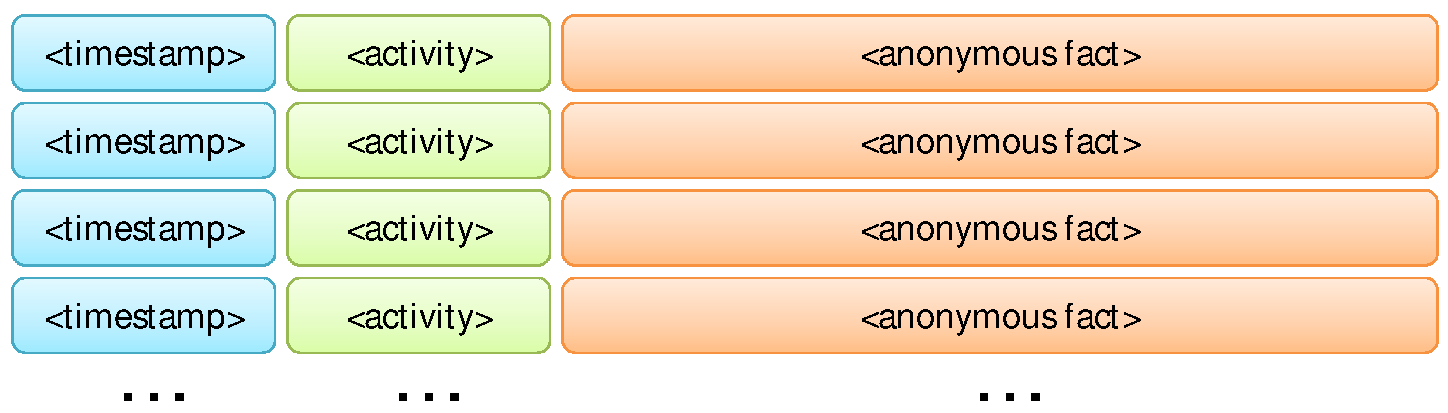
\includegraphics[width=1\columnwidth]{26Snipes_activityLogTheoretical.pdf}
\caption{Abstract model of developer activity streams.}
\label{fig:theoretical}
\end{figure*}



\subsection{Magnitude Analysis}

%advantages
A major advantage of anonymous usage data is the fact that it captures developers in their natural habitat, without any observational bias. Deriving conclusions from hours of developers' field work is naturally more convincing than from hour-long, in-laboratory developer studies. One type of questions that usage data is well-suited to answer uses measurement of the magnitude of occurrence of a specific event. For instance, researchers may want to know ``How often do developers invoke the pull-up refactoring'' or ``How often is the file search invoked?''. By performing a count of a specific message in the collected logs, researchers can easily calculate frequencies of specific actions that can be often sufficient to answer important research questions. 

%disadvantages
However, researchers must be wary of a few common issues with magnitude analysis. First, in any sufficiently large set of user logs there is a small set of developers that will use the feature/tool under analysis orders of magnitude more often than the general population, potentially skewing the data. 
Second, attempts to attribute time to individual activities are fraught with difficulties. For instance, there is a temptation to report the percentage of time spent doing activity X. Yet, because the data is based on a stream of activities any time calculation requires making unsound assumptions on what happens in between these events.

%Looked for an appropriate citing with Murphy as lead but did not find one. Not sure
%how else to cite a body of work from one person's perspective
Murphy et al's work on understanding Eclipse IDE usage provides several examples of magnitude analysis being used effectively. By simply counting instances of events in developers' activity streams they were able to present how often developers accessed certain views, the top 10 commands executed by developers, and the percentage of developers that used each specific refactoring command. In spite of the simplicity of this analysis its ideal for identifying heavily used features for improvements and unused features for removal, as well as for getting a sense of how developers are currently working. 

\subsection{Categorization Analysis}

%advantages
While magnitude analysis is well-suited for answering research questions about the use of a single IDE command, many research questions are related to a specific feature or tool in the IDE, which usually maps to multiple activities. For instance, the research question ``How often are refactorings performed?'' cannot be answered via magnitude analysis alone, as refactorings can be triggered through a number of different IDE commands. These commands first need to be categorized, after which magnitude analysis can be used. 

%disadvantages
When focusing on a concrete sub-task, such as refactoring, it may be easy to categorize activities. In this case, all refactoring commands, such as pull-up or extract method, can be classified as refactorings. However, when focusing on more general behavior, such as editing, navigating, and searching, categorization can be difficult. It is impossible to say, for instance, from a single click in the {\tt File Explorer} window, whether that click represents a search, as the developers browses a few promising files, or a navigation, as he implicitly opens a type declaration of a variable he was just browsing. Thus, categorization without context can produce noisy data in certain cases. However, categorization is a powerful tool, especially when there is little ambiguity in the IDE commands that are analyzed.

%example
To illustrate both the power and limitations of category analysis consider the following IDE data stream, and the research questions ``Do developers use code search tools?''. 
\begin{figure}
\hrulefill
\begin{verbatim}
Collector Started
2014-02-02 13:21:22 - User submitted query to Find-in-Files
2014-02-02 13:24:36 - Find-in-Files retrieved 42 results
2014-02-02 13:32:21 - User clicked on result 2
2014-02-02 13:46:56 - User submitted query to Quick Find
2014-02-02 14:07:12 - Open definition command; input=class
2014-02-02 14:46:52 - User submitted query to Find-in-Files
2014-02-02 14:46:56 - Find-in-Files retrieved 8 results
2014-02-02 14:48:02 - Click on File Explorer
\end{verbatim}
\hrulefill
	\caption{Log File Search Category Example}
	\label{log:logFileSearch}
\end{figure}


For this research question, the category of log events related to code search tools should be identified and counted. Modern IDEs commonly offer several code search tools, which operate at the global or local scale, such as the {\tt Find-in-Files} and {\tt Quick Find} tools.  An example log from Visual Studio with these tools is shown in Figure \ref{log:logFileSearch} based on Visual Studio. Using categorization analysis we can identify three
log events related to usage of code search tools, and report various statistics aimed at answering the research question (e.g., number of code search events per day, number of code search events per developer see figure \ref{fig:category}). However, the IDE usage data can sometimes be affected by noise, which cannot be avoided by categorization analysis. For instance, the second query to {\tt Find-in-Files} is not followed by a developer click, which is a failed interaction with the {\tt Find-in-Files} tool and should likely not be included in answering the research question.


\begin{figure*}[t]
\centering

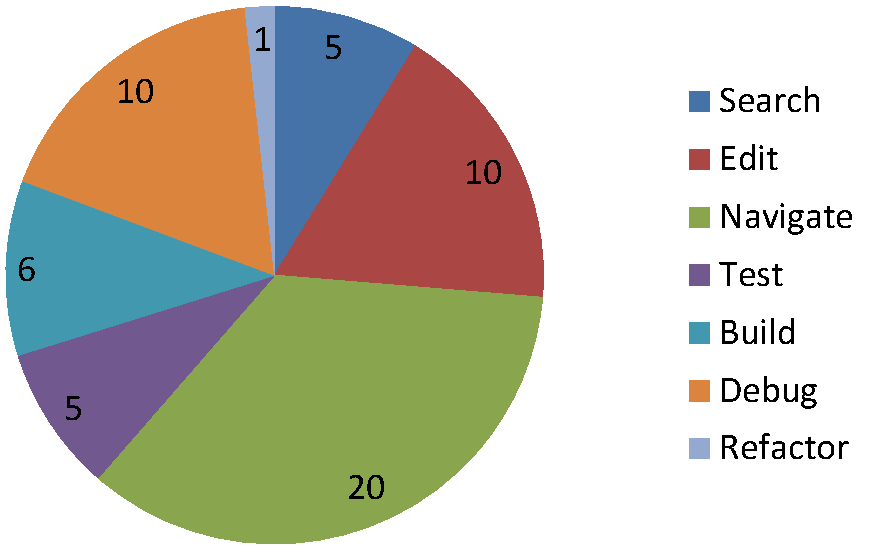
\includegraphics[width=0.5\columnwidth]{26Snipes_activityCategorization.pdf}
\caption{Categorized Log Events with Search Category}
\label{fig:category}
\end{figure*}


\subsection{Sequence Analysis}

%intro to sequence analysis
Magnitude analysis and categorization are both appropriate for answering research questions that are simply manifested in the IDE usage log. However, a more powerful way of analyzing activity logs is through sequence analysis, which first breaks the IDE data stream into a number of sequences, according to some criteria, and then reports upon characteristics of each sequence. A sequence in the IDE usage data corresponds to a software engineering task or sub-task accomplished by the developer (e.g. refactoring, looking for a starting point for a maintenance task, etc.), consisting of all of IDE events in a given time span. For instance, answering the research question of ``Are developers successful at finding initial points in the code for a software maintenance task?'' requires that the sequence of IDE events corresponding to each maintenance task be identified, before we can perform further analysis using either magnitude or categorization analysis. The granularity of a sequence is determined by the guiding research question. For certain research questions, we may be interested in a smaller sequences (e.g., searching the code base), while for others we may need to consider a longer time span (e.g., implementing a new feature, fixing a bug). 
According to ~\citeasnoun{Zou-ComanIndustry}, the larger and more complex the task or sub-task to extract, the harder it is for sequence analysis to determine its starting and stopping point in the activity log.

%how difficult or easy is it to determine sequences
In many cases, extracting activity sequences can be challenging as it impossible to know exactly when a developer begins or ends a particular task or sub-task, without understanding the developer's underlying thought process. There are several possibilities in how sequence extraction can be performed, based on the specific research question. One possibility is to use sentinels, which are specific actions that indicate the beginning and end of a sequence. For instance, in the context of the code search research question mentioned above, submitting a query to the code search tool begins a sequence, while performing an edit or structural navigation (e.g., following the call graph) ends the sequence. Another possibility is to use the passage of time to extract sequences, where time without any activity is used as a signal of task start or finish. Yet another possibility is to use locations in the code base to identify a sequence in the activity log. This is the key insight used in  ~\citename{Coman-TaskIdent}'s algorithm ~\citeyear{Coman-TaskIdent}, which uses periods of activity on the same program elements to represent the core of a task, and time distance between such events to extract sequences corresponding to developer tasks. In laboratory validation studies of this algorithm have shown very high accuracy (80\%) when compared to the ground truth reported by developers. ~\citeasnoun{Zou-ComanIndustry} find that this accuracy may not hold up in an industrial setting, where tasks are longer, code bases are more complex, and developer interruptions are common. Also, the algorithm requires that information regarding program elements is kept in the activity log, which may conflict with many developer's privacy and anonymity requirements.



\begin{figure}
\hrulefill
\begin{verbatim}
Collector Started
2014-02-02 13:46:52 - User submitted query to Find-in-Files
2014-02-02 13:46:56 - Find-in-Files retrieved 121 results
2014-02-02 13:52:21 - User clicked on result 2
2014-02-02 13:58:01 - User clicked on result 8
2014-02-02 13:59:57 - Open caller/callee command 
...
2014-02-02 14:46:52 - User submitted query to Find-in-Files
2014-02-02 14:46:56 - Find-in-Files retrieved 19 results
2014-02-02 15:01:08 - User clicked on result 11
2014-02-02 17:30:12 - User edited code
...
\end{verbatim}
\hrulefill
	\caption{Log File Sequence Example}
	\label{log:logFileSequence}
\end{figure}
%example
We illustrate sequence analysis with the usage log shown in Figure \ref{log:logFileSequence} and the research question  ``Are developers successful at finding initial points in the code for a software maintenance task?''
To answer the research question, sequence analysis can extract two separate sequences in the log from Figure \ref{log:logFileSequence} by using sentinels indicative of start/end of a code search activity, among other possible sequence identification approaches. Both of the extracted search sequences can be deemed as successful since for each of the queries to the {\tt Find-in-Files} code search tool the developer clicks on a retrieved result, followed by a structured navigation event (open caller/callee) or editing event (developer edited code). Therefore it would seem that the developer is successful at finding initial points in the code for his or her software maintenance task. However, on closer inspection of the second sequence, we observe that there is a large time gap between clicking on a result and editing code. The reason for this time gap is open to interpretation, as the developer may have returned to the previous results, continuing the search session, or have started on a completely new development activity. Certain types of sequence analysis, such as Coman's algorithm, take time into account when identifying sequences, while others, like the sentinel approach used above, do not. Neither of these approaches, however, helps to resolve the origin of ambiguous events, which are left to the researcher to characterize.

\subsection{State Model Analysis}

Another way to analyze log data is to view the log as a sequence of events occurring in a state machine.  Using state models, we can quantify the occurrences of repeating actions and describe a usage pattern in statistical analysis.  ~\citeasnoun{nagappan_logs_to_dags_tefse_2011} used sequence analysis to generate a graphical view of a profile of how users interacted with the components of a system from log data.  In state model analysis, the sequential data is converted to nodes and edges of a graph which represents the entire data in states and transitions between them.  A Markov state model provides information about the probability of occurrence of each state and the transitional probability of each activity.   The statistics provided in a Markov state model include the quantity of time and probability for the developer being in each state.  From a given state, the model calculates the probability of each transition to different unique states.  State models answer specific questions such as what is the probability that once a developer searches the code, they edit a code element listed in the find results. Expanding this question, the probability of an entire use case or set of transitions through the usage model, is calculable from the state model.  

State model graphs make it easy to identify the most active states and edges provides information about the important activities in the data set.  As the number of states increases, the WDG becomes more complex and hence difficult to understand.  When this occurs, summarizing the detailed event data into higher-level categories effectively combines the states to get more meaningful information.   For example, classifying events in usage data of similar types into categories results in fewer states with the same number of transitions as the original data.

We generate a state model from a usage log by transforming the serially ordered events in a sequence data to a Weighted Directed Graph (WDG) data structure.  We can abstract the information in the log line to any level, such as, event level, event category level, tool level, or application level. In the sequence data, each event is important as a standalone event, however, in the WDG representation, the importance shifts to adjacent pairs of events. 
%We do this type of a transformation to record the order in which events happened. 
Therefore, each unique event in the sequence data is represented by a unique node in the WDG. 

To understand how to interpret a state model, look at our example graph figure \ref{op-profile-example}.  We see that an edge exists from one node (head) to another (tail) if there is an occurrence of the event representing the tail node immediately after the event representing the head node in the  log file. For example if event B follows event A in the log file, then there is directed edge from node A to node B in the WDG. The edges are labeled with the number of times this transition has occurred.  For example if B occurs a fifty times after A in the log file, then the edge from node A to node B in the WDG is labeled with 50. Typically, we keep track of the actual count as the weight of the edge, when building the graph. In the graph we display the percentage value as the label. This percentage is proportional to the total number of transitions.  The cumulative probability of out-edges of a node is 1. The transitional probabilities of each out-edge is calculated by dividing the number of transactions of that out-edge with the sum of all outward transactions from that node. We could also store the dynamic parameter information in each log line as a list along the edges. 

As an example, consider a sample log file shown in figure \ref{samplelogfile} given below and the corresponding state model graph in figure \ref{op-profile-example}. Intuitively you can see how the state model represents the log states and transitions between them in the sequence of events.  

\begin{figure}
\hrulefill
\begin{verbatim}
2013-03-21 18:18:32Z,A
2013-03-21 18:18:33Z,B
2013-03-21 18:20:49Z,C
2013-03-21 18:20:50Z,A
2013-03-21 18:20:56Z,B
2013-03-21 18:20:57Z,A
2013-03-21 18:21:08Z,C
2013-03-21 18:21:08Z,D
2013-03-21 18:21:08Z,E
2013-03-21 18:21:08Z,A
\end{verbatim}
\hrulefill
\caption{Sample Log File to Convert to State Model}\label{samplelogfile}
\end{figure}

\begin{figure}[h]
  \centering
  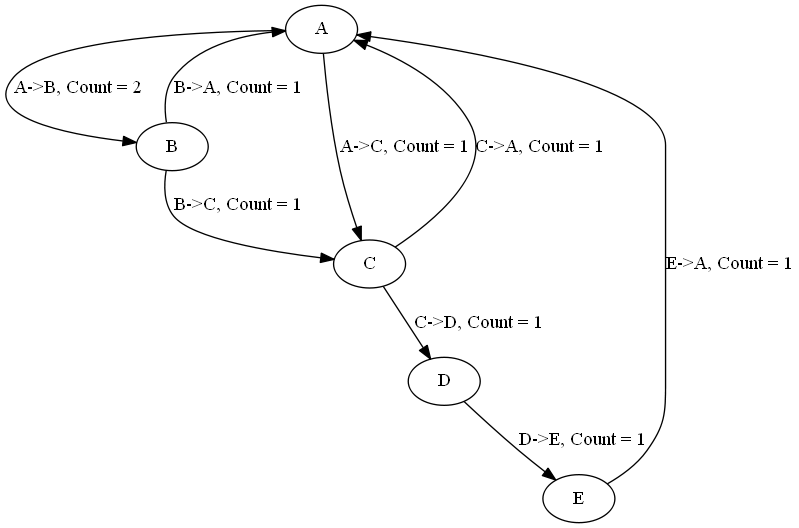
\includegraphics[scale=.40]{26Snipes_op-profile-example.png}
  \caption{Weighted Directed Graph of the Example Log}\label{op-profile-example}
\end{figure}






%the other example is aligned with the sample graph thus better.
%As an example of WDG, consider a simple log file where the activities are separated by commas. $1-2, 2-3, 3-4, 4-5, 5-4, 4-5, 5-4, 4-6, 6-7, 7-5, 5-4, 4-5, 5-4, 4-5, 5-8, 8-9$. The events in the log file are mapped to their corresponding event IDs: $1, 2, 3, 4, 5, 4, 5, 4, 6, 7, 5, 4, 5, 4, 5, 8, 9$. Each node is a unique event. An edge between nodes 1 and 2 signifies that the event 2  appears after event 1  in the log file. The labels on the edges have the actual count and could have the transitional probabilities as well. The transitional probability from node 1 to node 2 is 1.0, whereas the transitional probability from node 4 to node 6 is 0.2.  This is depicted in Fig \ref{op-profile-example}.
 
Converting a log into a state model requires three steps.  We use JUMBL (Java Usage Model Builder) from the Software Quality Research Laboratory (SQRL) of the University of Tennessee.    Details on input formats and JUMBL tools are available on sourceforge.\footnote{\url{http://jumbl.sourceforge.net/}}
\begin{enumerate}
\item
First, convert the log file into a representation for each transition called a sequence based specification. The format for a sequence based specficicaiton in csv files is described in the JUMBL user guide. This representation contains the following information with one row for each transition :
\begin{itemize}
\item State transition
\item Count of transitions
\item Total time elapsed
\item State In information
\item State Out information
\end{itemize}

\item
After importing the sequence based spec, JUMBL can write out the representation of a state model as a TML script or several other formats including GML (Graph Modeling Language) that graph tools can import.  The TML  has information about the nodes, the out edges from each node along with the number of transitions from each node to another. The corresponding graph for the usage log example is depicted in Fig. \ref{op-profile-example}
\end{enumerate}


Using state models, a sequence data with hundreds of thousands of lines can be quickly converted to more meaningful graphical representation using this method. Once the TML file is generated, we can use JUMBL to find out the state probabilities of each states. Using the state probability and the usage patterns we can draw conclusions about the occupancy of individual states and the use cases that involve transitions through several states.

%Trying this on without the following examples.  They don't really add much and raise more questions than they answer.  I hope reference take care of the how to in this case.


%
%\begin{figure}
%\label{sampleTML}
%\hrulefill
%\begin{verbatim}
%($ fill(1) $)
%model testlog
%//use this before each transition to show probability ($0.10$)
%
%source [A]
%($2$)"Count=2 (A->B), TimeElapsed= 7secs" [B]
%($1$)"Count=1 (A->C), TimeElapsed= 11secs" [C]
%
%[B]
%($1$)"Count=1 (B->C), TimeElapsed= 136secs" [C]
%($1$)"Count=1 (B->A), TimeElapsed= 1secs" [A]
%
%[C]
%($1$)"Count=1 (C->A), TimeElapsed= 1secs" [A]
%($1$)"Count=1 (C->D)" [D]
%
%[D]
%($1$)"Count=1 (D->E)" [E]
%
%[E]
%($1$)"Count=1 (E->A)" [A]
%
%
%"exit" [Exit]
%
%end 
%\end{verbatim}
%\hrulefill
%\caption{Sample TML for a State Model}
%\end{figure}



%%I commented these out because they were out in space in the document and not well supported by the text.  You probably cut the text because of other comments.  Anyhow does it make sense to stick with one WDG example based on the state model shown in text above?  Seems OK to me so far. 

 
\subsection{The Critical Incident Technique (CIT)}

The Critical Incident Technique (CIT) is a general methodology for improving a
process or system with respect to a set of objectives. CIT prescribes a
systematic study of the \emph{critical incidents}. Critical incidents are
\emph{positive} or \emph{negative} events that have a significant effect on the
objectives.

CIT was developed and published in its current form by Flanagan in
1954~\cite{Flanagan1954CIT}. Nevertheless, it is believed that the technique was
introduced even earlier by Galton (circa 1930). Variations of CIT have been
widely used in Human Factors~\cite{ShattuckWoods1994CIT}.

~\citeasnoun{DelGaldo1986CIT} applied CIT to Human-Computer Interaction (HCI) as part
of evaluating the documentation of a conferencing system.
They asked the study participants to perform a task and report any incident that
they ran into. The researchers observed the participants during the study,
analyzed the reported incidents, and proposed improvements to the documentation
accordingly.

In the context of IDEs, ~\citeasnoun{VakilianJohnson2014Alternate} adapted CIT to automated
refactorings. The goal of this study was to
identify the usability problems of automated refactorings by analyzing
refactoring usage data. The researchers found that certain events such as
cancellations, reported messages, and repeated invocations are likely indicators
of the usability problems of automated refactorings. By locating these events in
the usage data and analyzing their nearby events, the researchers were able to
identify 15 usability problems of the Eclipse refactoring tool. For instance,
the usage data indicated that six participants invoked the Move Instance Method
refactoring for a total of 16 times but none finished the refactoring
successfully. In all cases, the participants either canceled the refactoring or
could not proceed because of an error that the refactoring tool reported. By
inspecting these critical incidents, the researchers were able to infer two
usability problems related to Move Instance Method.

To apply CIT on a set of usage data, you should follow several steps. First,
identify the objectives. Finding usability problems is only one example.
Second, identify a set of events that may be critical incidents. These are
events they may have significant effects on your objectives. Usually, the
negative critical incidents, which may have negative effects on the objectives,
are better indicators of problems than the positive ones. Third, identify the
critical incidents in your usage data. Fourth, collect sufficient contextual
information to interpret the critical incidents. This may include events that
have occurred in close time proximity to the critical incidents. You may even
have to interview the developers or ask them to report their explanations of the
incidents during the study. Although the developer reports may be short or
incomplete, they can provide more insight about the nature of the problems.
Finally, evaluate the effectiveness of the critical incidents and revisit the
steps above. The process that we described for applying CIT on usage data is
iterative in nature. That is, it is natural to go back to a previous step from
each step.

\label{sec:IncludingOtherSources}
\subsection{Including Data From Other Sources}


Other data sources, such as developer feedback, task descriptions, change histories can provide context for usage data and yield new opportunities for supporting developers. In this section, we briefly outline some related work in this area.

\subsubsection{Developer Feedback}

Usage data collection can be augmented by explicit developer feedback to establish a ground truth. For instance, if you want to understand a developer's opinion of a tool or his or her purpose for using an IDE feature, it is best to ask about it. A post-analysis interview can shed light on your observations and confirm your analysis or point out different aspects.

Information on a developer's activities can provide an additional rational to the usage data and explain the developer's actions. Asking questions on how well the developer knows the code he or she is working on can explain a developer's navigation patterns and usage of code search~\citeaffixed{SnipesExperiencesGamifyingSoftwareDevelopment}{e.g.,}, while questions on the task, e.g., implementing a new feature versus fixing a bug, can explain other characteristics, such as the amount of editing versus testing.

\subsubsection{Tasks}

As mentioned above, Mylin is a popular extension to the Eclipse IDE that supports task
management, reducing the effort for a developer to switch between
tasks and maintaining relevant information for each
task~\cite{Kersten-Mylyn}. In the context of a specific task, Mylin
collects usage data in order to compute a degree-of-interest (DOI)
value for each program element, which represents the interest the
developer has in the program element for the task at hand. Program elements that a developer interacted with frequently and recently have a higher DOI value. Using these calculated DOI values, Mylyn highlights the elements relevant for the current task and filters unnecessary information from common views in the IDE. 

\subsubsection{Change History}

The FastDash tool by ~\citeasnoun{FastDash} enables real-time awareness of other developers'
actions (e.g., focus or edits to a specific file) by utilizing usage
data in concert with the source files and
directories. FastDash's purpose is to reduce faults
caused by lack of communication and lack of awareness of activities
that other developers are performing on the same code base. The tool
highlights other developer's activity as it is occurring using a
sophisticated dashboard on the developer's screen or on a team's dashboard.






\vspace{0.1in}
Using this overview of analysis techniques should give you a good start towards analyzing usage data for your research.
The ideas you bring to your usage data analysis process provide the real opportunities for innovating usage data based research.  Next we will discuss limitations we have observed in conducting research with usage data.

\section{Limits of What You Can Learn from Usage Data}
\label{sec:limitations}

Collecting usage data is potentially a boon to research, and as we have
pointed out, has many interesting and impactful applications.
Nonetheless, there are limits to what you can learn as a researcher
from usage data.
In fact, our experience is that researchers (and practitioners) have
high expectations about what they can learn from usage data, and those
expectations often come crashing down after significant effort implementing
and deploying a data collection system.
So before you begin your usage data collection and analysis, consider
the following two limitations of usage data.

\textbf{Rationale is Hard to Capture.}
Usage data tells you what a software developer did, but not
why she did it.
For example, if your usage data tells you that a developer used
new refactoring tool for the first time, from a trace alone you cannot determine whether
(a) she learned about the tool for the first time, (b) she had used the tool earlier, but before you started collecting data, or (c) her finger slipped and she pressed a hotkey by accident. We do not know whether she is satisfied with the the tool and will use it again in future.
A researcher may be able to distinguish between these by collecting additional information,
like asking the developer just after she used the tool why she used it,
but it is impossible to definitively separate these based on the
usage data alone.

\textbf{Usage Data Never Captures Everything.}
Researchers often want to capture ``everything,'' or at least
everything that a developer does.
This is fundamentally impossible, and the reason we introduced the
goal-question metric.
If you have a system that captures all key presses, you are still
lacking information about mouse movements.
If you have a system that also captures mouse movements, you're still
missing the files that the developer is working with.
If your system captures also the files, you still lacking the
histories of those files.
And so on.
Ultimately, usage data is all about fitness for purpose -- is the data
you are analyzing fit for the purpose of your research questions.

To avoid these limitations, we recommend thinking systemically about how the data will be used while planning rather than thinking about usage data collection abstractly.
Invent an ideal usage data trace, and ask yourself:

\begin{itemize}[noitemsep]
  \item Does the data support my hypothesis?
  \item Are there alternative hypotheses that the data would support?
  \item Do I need additional data sources?
  \item Can the data be feasibly generated?
\end{itemize}

\noindent
Answering these questions will help you determine whether you can sidestep
the limitations of collecting and analyzing usage data.

\section{A Look Ahead}

If the last two decades could be labeled the era
of big data collection,
the next two decades will surely be labeled as the
era of smarter big data analysis.
Many questions still remain:
How do we balance data privacy and data richness?
What are the long term effects of developer monitoring?
How can we maximize the value of data collection
for as many researchers as possible, and reduce the
strain on research participants? How can we provide right data to right person at right time with the least effort?
Answering these questions will help our research
community advance in usage data collection and analysis.

Usage data, while now widely collected, still remains largely
an untapped resource by practitioners and researchers.
In this chapter, we have explained how to collect and
analyze usage data, which we hope will help you ``stand
on the shoulders of giants'' and increase the ease
with which you can collect and analyze your own usage data.

% LocalWords: IDE IDEs UDC refactoring refactorings

\section{Code Listings}
The following code listings show the code for Build It Yourself for Visual Studio in section \ref{buildItYourself}.

Listing for DataRecorder.cs
\lstinputlisting[caption=DataRecorder,  breaklines=true,  label=code:DataRecorder_4]{VisualStudioMonitor/Monitor/DataRecorder.cs}

\newpage
Listing for AbstractMonitoredEvent.cs
\lstinputlisting[caption=AbstractMonitoredEvent,  breaklines=true, label=code:AbstractMonitoredEvent_4]{VisualStudioMonitor/Monitor/AbstractMonitoredEvent.cs}

\newpage
Listing for MonitoredCommandEvent.cs
\lstinputlisting[caption=MonitoredCommandEvent, breaklines=true,  label=code:MonitoredCommandEvent_4]{VisualStudioMonitor/Monitor/MonitoredCommandEvent.cs}

\newpage
Listing for MonitoredEventFactory.cs
\lstinputlisting[caption=MonitoredEventFactory, breaklines=true,  label=code:MonitoredEventFactory_4]{VisualStudioMonitor/Monitor/MonitoredEventFactory.cs}

\newpage
Listing for MonitoredEventCollection.cs
\lstinputlisting[caption=MonitoredEventCollection,  breaklines=true, label=code:MonitoredEventCollection_4]{VisualStudioMonitor/Monitor/MonitoredEventCollection.cs}



\bibliographystyle{abbrv}
\bibliography{26Snipes_Bibliography} 


\end{document}
